\documentclass[12pt]{article}

\usepackage[UTF8]{ctex}
\usepackage{appendix}
\usepackage{enumerate}
\usepackage{amsmath}
\usepackage{graphicx}
\graphicspath{{picture/}}
\usepackage{longtable}
\usepackage{cite}
\usepackage{zhnumber}
\usepackage{array}
\usepackage{bigstrut}
\usepackage{geometry}
\geometry{left =2.5 cm,right=2.5cm,top=2.5cm,bottom=2.5cm}
\usepackage{multirow}
\usepackage{lastpage}
\usepackage{longtable}
\usepackage{listings}
 \usepackage{color}
  \usepackage{xcolor}
 \lstset{
  language=Matlab,  %代码语言使用的是matlab
  rulesepcolor=\color{red!20!green!20!blue!20},%代码块边框为淡青色
  keywordstyle=\color{blue!90}\bfseries, %代码关键字的颜色为蓝色,粗体
    numbers=left, % 显示行号
    numberstyle=\tiny,    % 行号字体
   commentstyle=\color[RGB]{0,130,0},    % 设置代码注释的颜色
  showstringspaces=false,%不显示代码字符串中间的空格标记
  stringstyle=\ttfamily, % 代码字符串的特殊格式
  breaklines=true, %对过长的代码自动换行
  extendedchars=false,  %解决代码跨页时,章节标题,页眉等汉字不显示的问题
  escapeinside=``,      % 代码中出现中文必须加上,否则报错
  texcl=true,}
  \lstset{breaklines}
\usepackage[section]{placeins}
\usepackage[colorlinks,linkcolor=blue]{hyperref}
\usepackage{titlesec}
\usepackage{titletoc}
\titleformat{\section}{\centering\heiti\zihao{3}}{实验\zhnum{section}}{0.3em}{}
\titleformat{\subsection}{\heiti \fontsize{12pt}{0}}{\thesubsection}{0.3em}{}
\renewcommand\figurename{\heiti\zihao{5} 图}
\renewcommand\tablename{\heiti\zihao{5} 表}
\renewcommand {\thetable} {\thesection{}.\arabic{table}}
\renewcommand {\thefigure} {\thesection{}.\arabic{figure}}
\renewcommand {\theequation} {\thesection{}.\arabic{equation}}
\usepackage{caption}
\captionsetup[figure]{labelsep=space}
\captionsetup[table]{labelsep=space}
\date{}
\geometry{a4paper,scale=0.8}

\begin{document}%文档从这里开始。

\numberwithin{footnote}{section}
\renewcommand{\contentsname}{\centering 目录}
\renewcommand{\tablename}{表}
\renewcommand{\figurename}{图}
\renewcommand\refname{参考文献}
\renewcommand\appendix{\setcounter{secnumdepth}{0}}
\renewcommand\abstractname{摘要}
\begin{figure}[h]
  \centering
  
\includegraphics[width=.6\textwidth]{logo}
\end{figure}
\thispagestyle{empty}
\begin{center}
\zihao{0}\heiti{雷达信号处理}\\
\zihao{0}\heiti{实验报告}\\\ \\\
\zihao{3}
\begin{songti}
\\ \
\renewcommand\arraystretch{1.5}
\begin{tabular}{p{1.5cm}<{\centering} p{0.2cm}<{\centering} p{3.5cm}<{\centering} p{1.5cm}<{\centering} p{0.2cm}<{\centering} p{3.5cm}<{\centering}}
组员&\textbf{:}&\kaishu{许晓明}&学号&\textbf{:}&9161040G0734\\\cline{3-3}\cline{6-6}
组员&\textbf{:}&\kaishu{周世峰}&学号&\textbf{:}&916104330154\\\cline{3-3}\cline{6-6}
学院&\textbf{:}&\multicolumn{4}{c}{\kaishu{电子工程与光电技术学院}}\\\cline{3-6}
专业&\textbf{:}&\multicolumn{4}{c}{\kaishu{电子信息工程}}\\\cline{3-6}
题目&\textbf{:}&\multicolumn{4}{c}{\kaishu{雷达信号处理}}\\\cline{3-6}
 & &\multicolumn{4}{c}{\kaishu{实验报告}}\\\cline{3-6}
教师&\textbf{:}&\multicolumn{4}{c}{\kaishu{张文青}}\\\cline{3-6}
\end{tabular}
\end{songti}
\end{center}
\begin{table}[b]
  \centering\zihao{3}
\number\year\ 年\ \number\month月
\end{table}

\begin{center}
\newpage
%\raggedright
\zihao{4}
\newpage
\pagenumbering{Roman}
\setcounter{page}{1}
\tableofcontents
\newpage
\pagenumbering{arabic}
\setcounter{page}{1}

\end{center}

\setcounter{page}{1}
\section{正交相干检波器}
\setcounter{equation}{0}
\setcounter{table}{0}
\setcounter{figure}{0}
在雷达信号处理中,由于信号与干扰混合波形的振幅和相位均含有信息,因此对信号最佳处理应在接收机的中频进行。但是,对信号进行数字处理时,在中频进行采样是很困难的。由于中频本身并无目标信息,目标信息包含在中频的复包络中。因此,须将中频信号变成等效的复数视频信号,以利于用数字处理。正交相干检波器就是一种将中频信号变换成复数视频信号的装置。
\subsection{实验目的}
\begin{enumerate}
  \item 掌握正交相干检波的基本原理,实现方法和运用它检测信号(例如多普勒 信号)。
\item 掌握正交相干检波器幅度一致性和相位正交性(幅度不平衡度)的测量方 法。
\end{enumerate}
\subsection{实验仪器}
信号源、示波器、直流稳压电源
\subsection{实验原理}
本实验的原理方框图如图\ref{zjxgylKT1}
所示。\par
\begin{figure}[htbp]
  \centering
  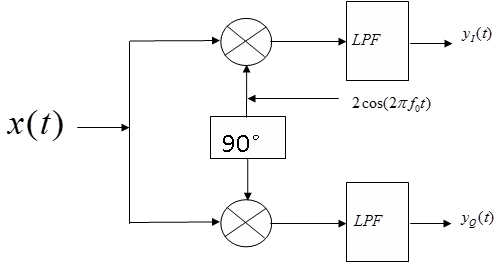
\includegraphics[width=0.5\textwidth]{word/0012}
  \caption{正交相干检波器原理方框图}\label{zjxgylKT1}
\end{figure}
假定图\ref{zjxgylKT1}中输入的实窄带信号为:
\begin{equation}
x(t)=a(t)\cos[2\pi f_0 t+\varphi(t)]
\end{equation}
其中,$a(t)$为实窄带信号的幅度调制;�$f_0$为实窄带信号的中频$\varphi�(t�)$为实窄带信号的相位调制。如果$x(t)$用复指数表示,可写成:
\begin{equation}
  x(t)=a(t)e^{j\varphi(t)}e^{j 2\pi f_0 t}=\mu(t)e^{j 2\pi f_0 t}
\end{equation}
其中,$\mu(t)=a(t)e^{j\varphi (t)}$是复包络, $e^{j2\pi f_0 t}$是复载频。\par
$x(t)$中的信息全部包含在复包络$\mu (t)$中,所以只要处理$\mu (t)$就可以得到信号的全部信息。复包络$\mu (t)$可进一步写成:
\begin{equation}
 \mu (t)=a(t)e^{j\varphi (t)}=a(t)cos\varphi (t)+ja(t)sin\varphi (t)
\end{equation}
参见图\ref{zjxgylKT1},I支路乘法器的输出为:
\begin{equation}
 x(t)x_L (t)=2a(t)\cos[2πf_0t+\varphi (t)]\cos(2\pi f_0t)=a(t)\left(\cos\varphi (t)+\cos[4\pi f_0 t+\varphi(t)] \right)
\end{equation}
经过低通滤波(LPF)后输出为:
\begin{equation}
y_I(t)=a(t)cos\varphi(t)
\end{equation}
同样,Q支路乘法器经过低通滤波(LPF)后输出为:
\begin{equation}
y_Q(t)=a(t)\sin\varphi (t)
\end{equation}
用$y_I(t)$ 作为实部, $y_Q(t)$作为虚部,组成一复信号恰好是中频 $x(t)$的复包络,即:
\begin{equation}
\mu (t)=y_I(t)+jy_Q(t)
\end{equation}
因$y_I(t)$和 $y_Q(t)$均为视频信号,而且包含了原信号的幅度和相位
\begin{equation}
\left\{
\begin{array}{c}
a(t)=\sqrt{(y^2_I(t)+y^2_Q(t))}\\
\varphi(t)=tg^{-1}\frac{y_Q (t)}{y_I (t)}\\
\end{array}\right.
\end{equation}
经变换后,就可对信号进行数字处理。
\subsection{实验步骤}
\begin{enumerate}
  \item 连接实验装置;
  \item 幅相不平衡度测量方法;
  \begin{enumerate}[(1).]
    \item 从示波器上读取正交I、Q信号的电压幅度值为$A_I$和$A_Q$,按公式:
    \begin{equation}
\Delta A=20\lg\frac{A_I}{A_Q}(dB)
    \end{equation}
        计算幅度平衡值。
  \item 测量TA和TB的值,按公式:
  \begin{equation}
 \Delta \varphi =\left|\frac{TA-TB}{TA+TB}\right|\times 90^\circ
  \end{equation}
    计算相位平衡度。
  \end{enumerate}
  \item 记录波形;
  \item 测数据;
\end{enumerate}
\subsection{实验结果}
\subsubsection{波形记录}
各类输出波形情况见表\ref{tab:fdphxwph122}。
\begin{longtable}{|c|c|c|}
    \caption{正交相干检波器波形记录}
    \label{tab:fdphxwph122}\\
    \hline
    符号&含义&波形\\
    \hline
    \endfirsthead

    \hline
    符号&含义&波形\\
    \hline
    \endhead

    \hline
    \endfoot

    \hline
    \endlastfoot

      QQ & Q路输出(LPF后) &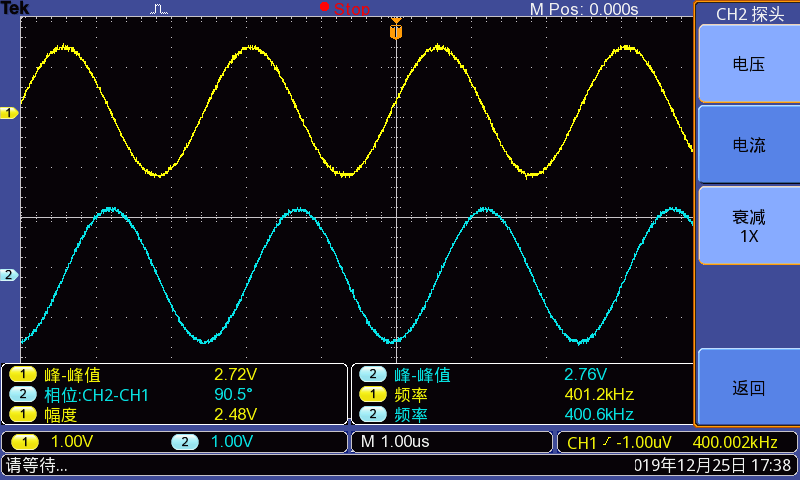
\includegraphics[width=0.45\textwidth]{data3/new/F0000TEK} \\
    \hline
    II & I路输出(LPF后) &同上,黄色为Q路输出,蓝色为I路输出  \\
    \hline
    Q & Q路输出(LPF前) &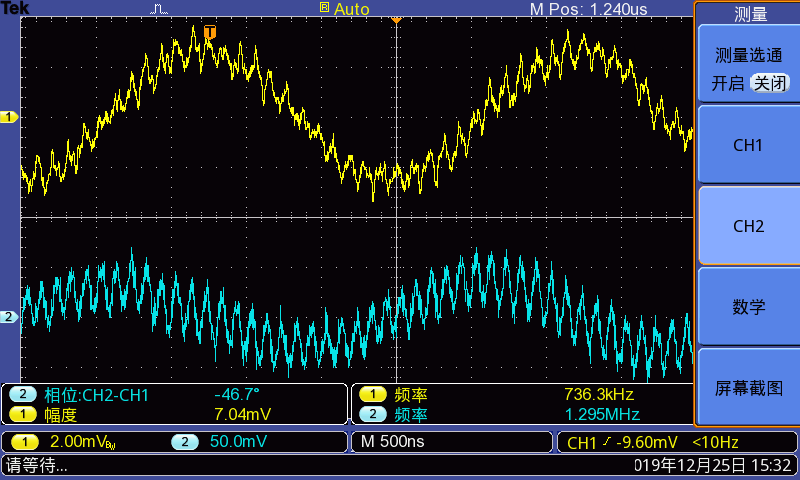
\includegraphics[width=0.45\textwidth]{data3/new2/F0011TEK}  \\
    \hline
    I & I路输出(LPF前) & 同上,黄色为Q路输出,蓝色为I路输出 \\
    \hline
    /FO & 中频正交本振 & 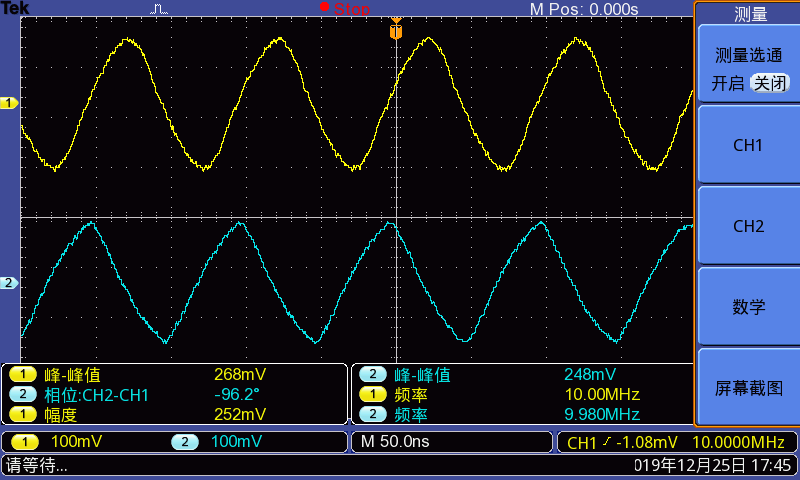
\includegraphics[width=0.45\textwidth]{data3/new/F0008TEK} \\
    \hline
    FO & 中频本振 & 同上,黄色为中频正交本振,蓝色为中频本振 \\
    \hline
    IN & 中频输入信号 & 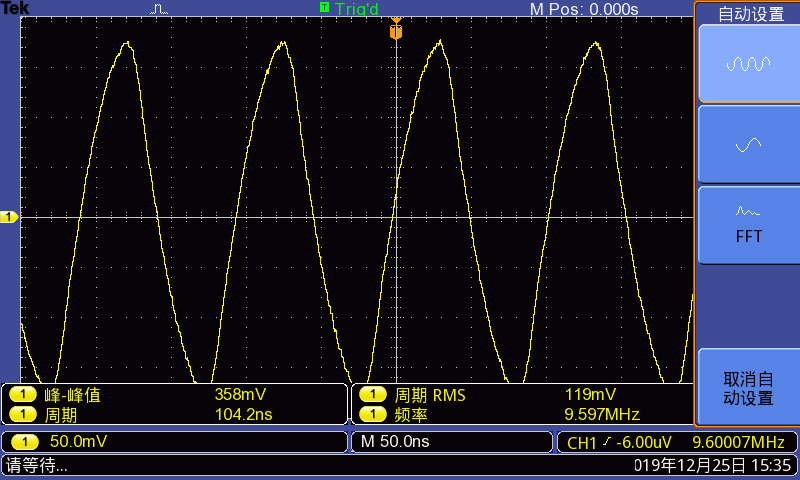
\includegraphics[width=0.45\textwidth]{data3/new2/F0013TEK}  \\
\end{longtable}
\subsubsection{幅度平衡与相位平衡}
在计算相位平衡情况时,首先易知两路波形的周期应当一致,设为$T$;再设两路波形的相位差为$\Delta\phi$(单位:度),则$TA={\frac{\Delta\phi}{360^\circ}\cdot T}$,$TB=\frac{T}{2}-TA={\frac{180^\circ-\Delta\phi}{360^\circ}\cdot T}$,化简相位平衡度计算公式可得:
\begin{equation}
\begin{array}{rl}
 \Delta\varphi&=\left|\frac{TA-TB}{TA+TB}\right|\times 90^\circ \\
 &=\left|\frac{{\frac{\Delta\phi}{360^\circ}\cdot T}-{\frac{180^\circ-\Delta\phi}{360^\circ}}\cdot T}{{\frac{\Delta\phi}{360^\circ}\cdot T}+{\frac{180^\circ-\Delta\phi}{360^\circ}}\cdot T}\right|\times 90^\circ \\
 &=\left|\frac{2\Delta\phi-180^\circ}{180^\circ}\right|\times 90^\circ \\
 &=\left|\frac{2\Delta\phi-180^\circ}{180^\circ}\times 90^\circ\right| \\
 &=\left|\frac{2\Delta\phi-180^\circ}{2}\right|  \\
  &=\left|{\Delta\phi-90^\circ}\right|  \\
  &=\left|90^\circ-\Delta\phi\right|  \\
\end{array}
\end{equation}
即,\textbf{\textcolor[RGB]{255,0,0}{可以通过计算两路波形相位差与$90^\circ$的差来得到相位平衡度}},而
幅度平衡与相位平衡数据见表\ref{tab:addlabelfxbphd1}。\par
\begin{table}[htbp]
  \centering
  \caption{正交相干检波器幅度平衡与相位平衡测试数据}
    \begin{tabular}{|c|c|c|c|c|c|c|c|c|}
    \hline
    输入频率(MHz) & 9.6 & 9.7 & 9.8 & 9.9 & 9.95 & 9.97 & 9.99 & 9.999 \\
    \hline
    检波器输出频率(KHz) & 400.6 & 300 & 199.4 & 100.2 & 49.9 & 29.94 & 9.99 & 1 \\
    \hline
    $\Delta A $幅度平 衡(dB) & -0.1268 & 0 & -0.0993 & -0.0949 & -0.1848 & -0.091 & -0.09 & -0.091 \\
    \hline
    $\Delta j $相位平 衡($ ^\circ$) & 0.5 & 0.8 & 1 & 1.3 & 0.2 & 2.9 & 1.2 & 2.2 \\
    \hline
    \end{tabular}%
  \label{tab:addlabelfxbphd1}%
\end{table}%
对应的波形情况如表\ref{tab:fdphxwph2}
。
% Table generated by Excel2LaTeX from sheet 'Sheet1'
\begin{longtable}{|c|c|}
    \caption{正交相干检波器幅度平衡与相位平衡波形}
    \label{tab:fdphxwph2}\\
    \hline
    输入频率(MHz)&波形\\
    \hline
    \endfirsthead

    \hline
    输入频率(MHz)&波形\\
    \hline
    \endhead

    \hline
    \endfoot

    \hline
    \endlastfoot

    9.6 & 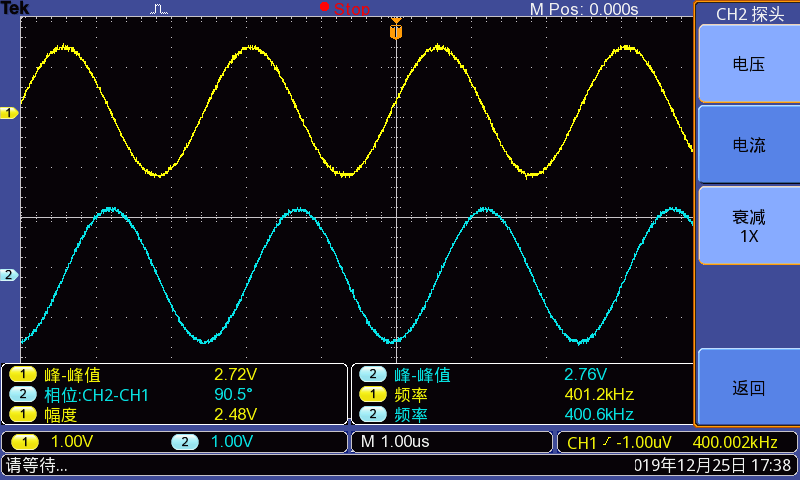
\includegraphics[width=0.45\textwidth]{data3/new/F0000TEK} \\
    \hline
    9.7 & 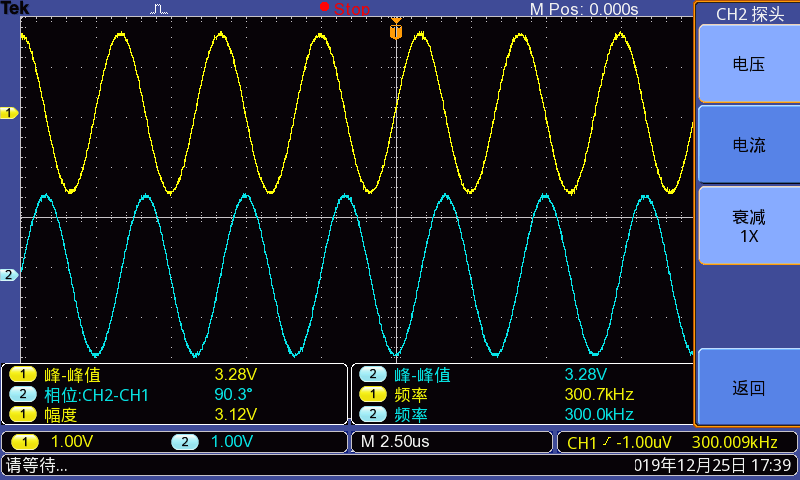
\includegraphics[width=0.45\textwidth]{data3/new/F0001TEK} \\
    \hline
    9.8 &  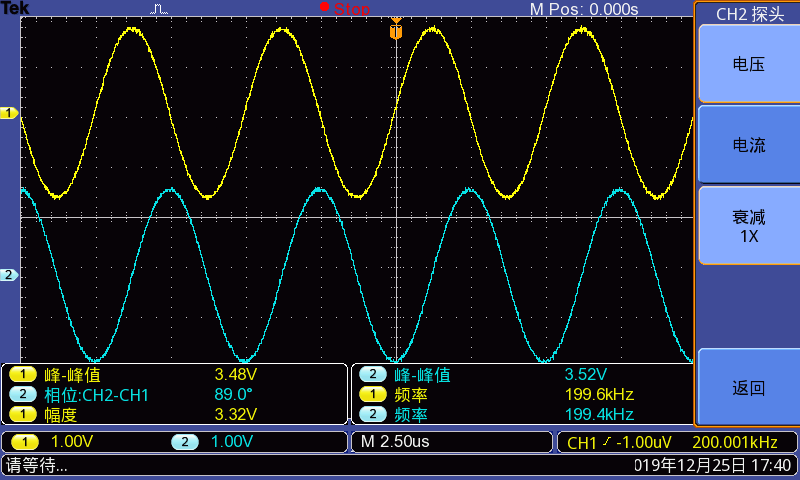
\includegraphics[width=0.45\textwidth]{data3/new/F0002TEK}\\
    \hline
    9.9 & 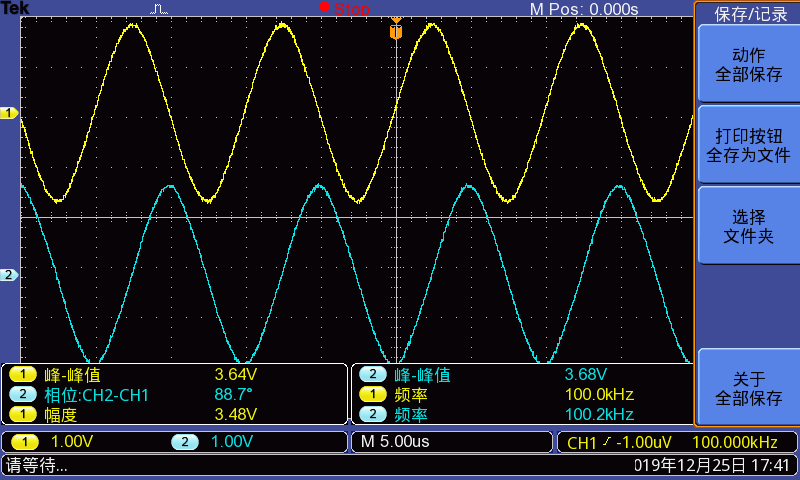
\includegraphics[width=0.45\textwidth]{data3/new/F0003TEK} \\
    \hline
    9.95 &  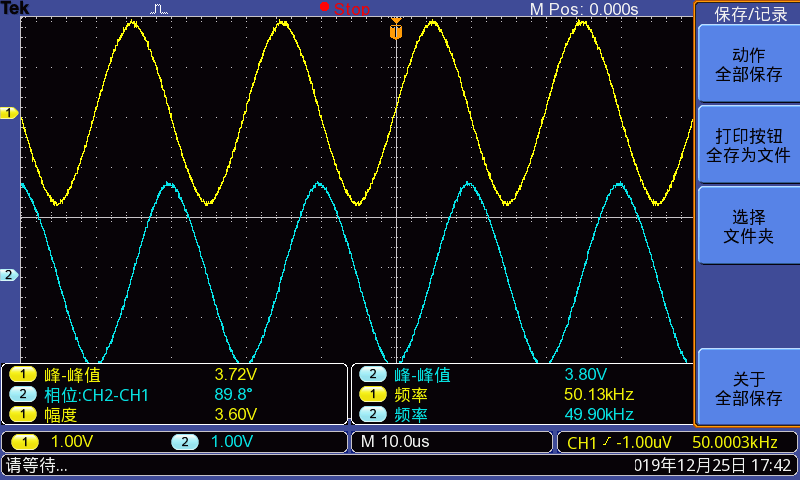
\includegraphics[width=0.45\textwidth]{data3/new/F0004TEK}\\
    \hline
    9.97 &  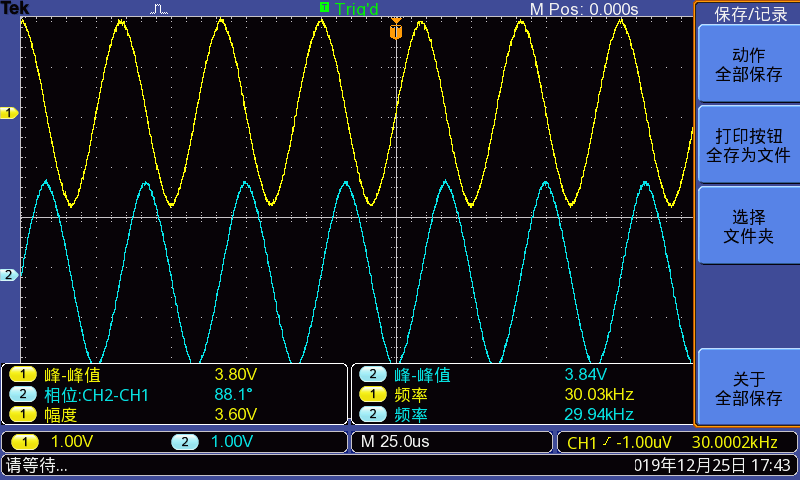
\includegraphics[width=0.45\textwidth]{data3/new/F0005TEK}\\
    \hline
    9.99 & 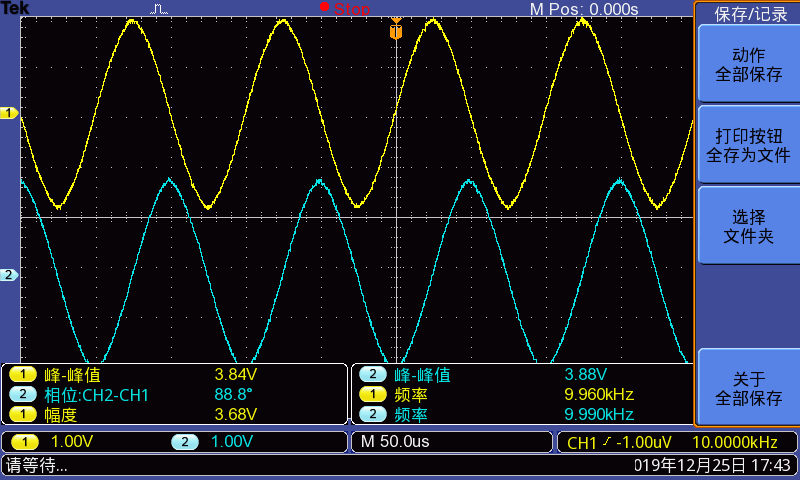
\includegraphics[width=0.45\textwidth]{data3/new/F0006TEK} \\
    \hline
    9.999 & 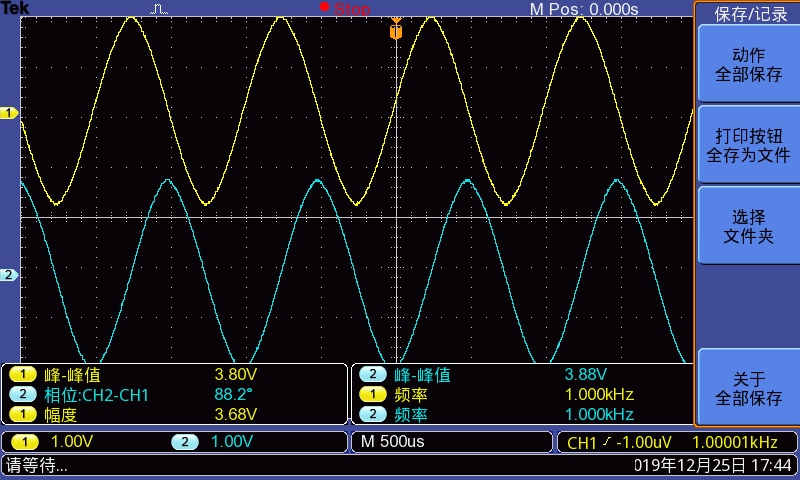
\includegraphics[width=0.45\textwidth]{data3/new/F0007TEK} \\
\end{longtable}
\subsubsection{中频本振幅相不平衡度}
中频本振幅相不平衡度数据见表\ref{tab:addlabel1112},对应的波形如图\ref{ZJXGJTQZPXHFXBPHD1}
所示。

\begin{table}[htbp]
  \centering
  \caption{正交相干检波器中频本振幅相不平衡度测试数据}
    \begin{tabular}{|c|c|c|}
    \hline
    性能 &$\Delta A $幅度平 衡(dB) &$\Delta j $相位平 衡($ ^\circ$)  \\
    \hline
    数据 & -0.6737 & 6.2 \\
    \hline
    \end{tabular}%
  \label{tab:addlabel1112}%
\end{table}%
\begin{figure}[htbp]
  \centering
  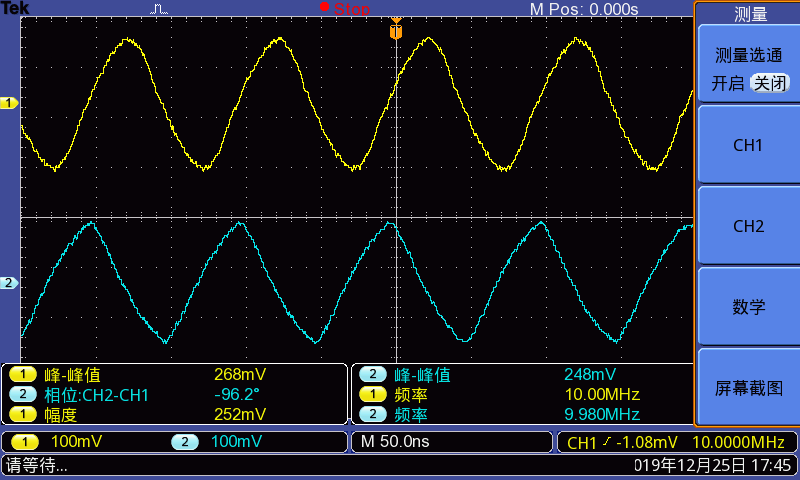
\includegraphics[width=0.5\textwidth]{data3/new/F0008TEK}
  \caption{正交相干检波器中频本振幅相不平衡度波形}\label{ZJXGJTQZPXHFXBPHD1}
\end{figure}
\subsection{思考题解答}
\begin{enumerate}
  \item \textbf{幅相不平衡是什么原因造成的?}\par
  模拟移相器输出正交的sin和cos信号很难完全保证幅度完全相同,相位相差90度,使得输出信号存在误差;同时,实验中解调后,还需低通滤波、放大处理,由于模拟滤波器和放大器不可能做到电路元件参数完全一致,再加上温度等外界环境的影响,出现误差。
\item \textbf{幅相不平衡如何进行调整?}\par
可以采用误差校正技术。接收机在检波前注入一个已知的理想信号,该号必须是已知其特性的合成多普勒信。经检波和处理后输出的信号可以反应检波器的幅相不平衡情况,对这个信号进行误差数据分析并整理出校正信息,则可在后续系统工作时,借助校正信息实现校正。
\item \textbf{不同频率下为什么幅相不平衡度不一致?}\par
由于两通道的元器件是有源的,在不同频率下的偏差不一致,使得不同频率下幅相不平衡度不一致。
\end{enumerate}
\newpage
\section{匹配滤波器}
\setcounter{equation}{0}
\setcounter{table}{0}
\setcounter{figure}{0}
\subsection{实验目的}
\begin{enumerate}
  \item 了解匹配滤波器的工作原理。
\item 掌握二相编码脉压信号的压缩比、主旁瓣比、码元宽度的测量方法。
\item 加深和巩固课堂所学有关距离分辨力、横向滤波器和匹配滤波方面知识。
\end{enumerate}
\subsection{实验仪器}
示波器、直流稳压电源、万用表。
\subsection{实验原理}
二相编码信号的匹配滤波器为:
\begin{equation}
 H(f)=\mu_1(f)\cdot\mu_2(f)
\end{equation}
式中, $\mu_1(f)$为子脉冲匹配滤波器, $\mu_2 (f)$为横向滤波器(即抽头加权延时线求和网络)。二相编码信号的匹配滤波器结构如图\ref{PPLVQKT1}
所示。\par
\begin{figure}[htbp]
  \centering
  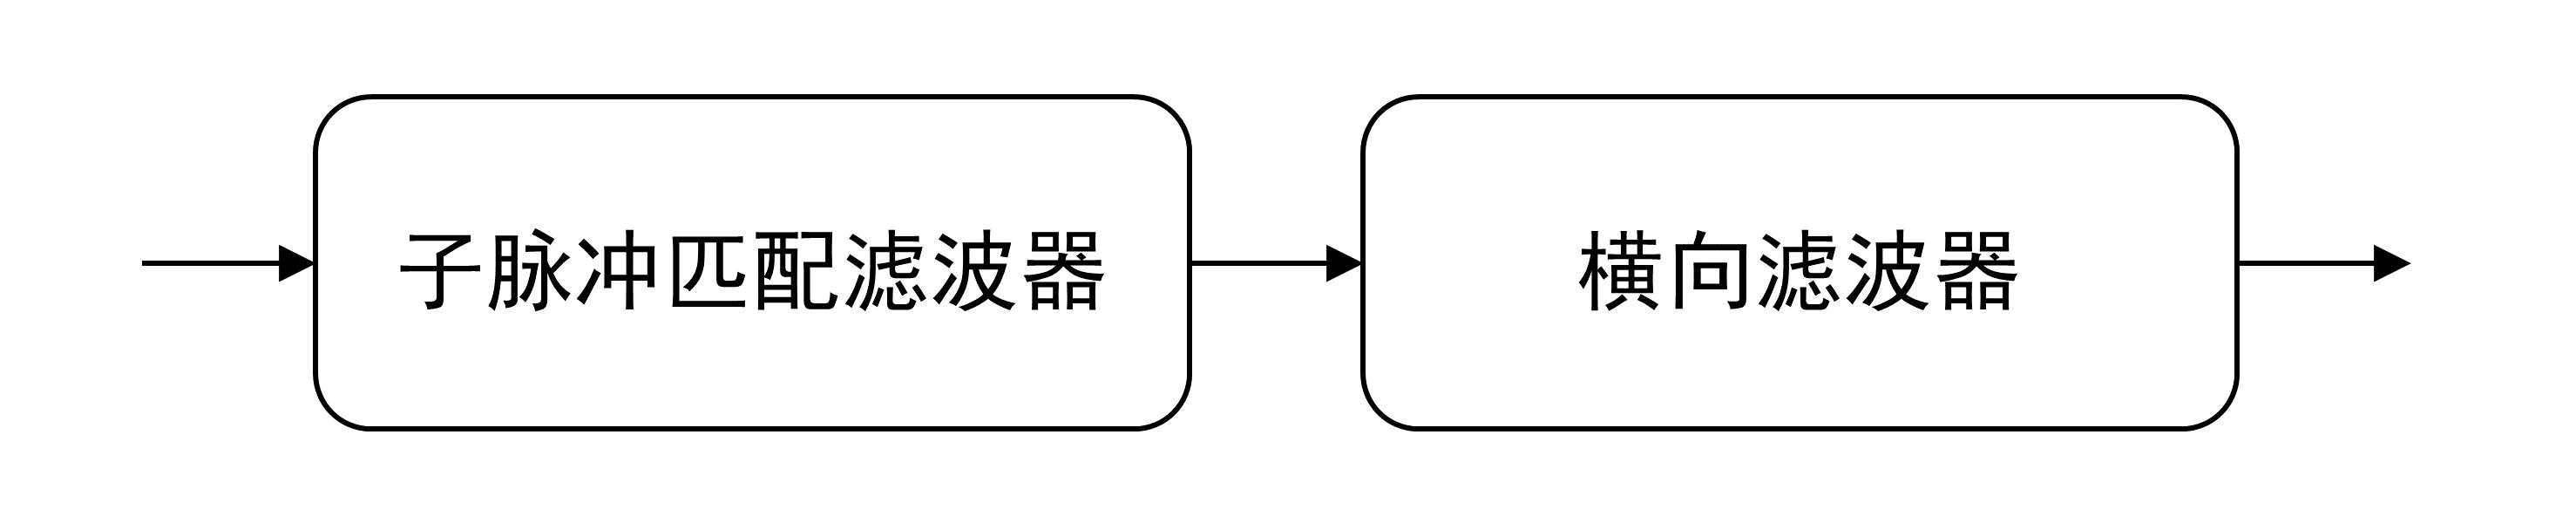
\includegraphics[width=0.5\textwidth]{PPT/4}
  \caption{二相编码信号的匹配滤波器结构}\label{PPLVQKT1}
\end{figure}
子脉冲匹配滤波器频率特性为:
\begin{equation}
  \mu_1 (f)=\sqrt{\frac{T}{P}}sinc(fT)e^{j\pi fT}
\end{equation}\par
横向滤波器频率特性为:
\begin{equation}
\mu_2(f)=\sum_{k=0}^{p-1}c_{(p-1)-k}e^{-j2\pi f(KT)}
\end{equation}
式中,P为码长;T为码元宽度;CK为二相编码信号。\par
在此,采用数字信号处理省略了子脉冲匹配滤波器,所以脉压输出不再是三角波而是方波。
横向滤波器(即抽头加权延时线求和网络)的结构如图\ref{HXCTJQYSX}
所示, 在此采用超大规模集成电路完成。
\begin{figure}[htbp]
  \centering
  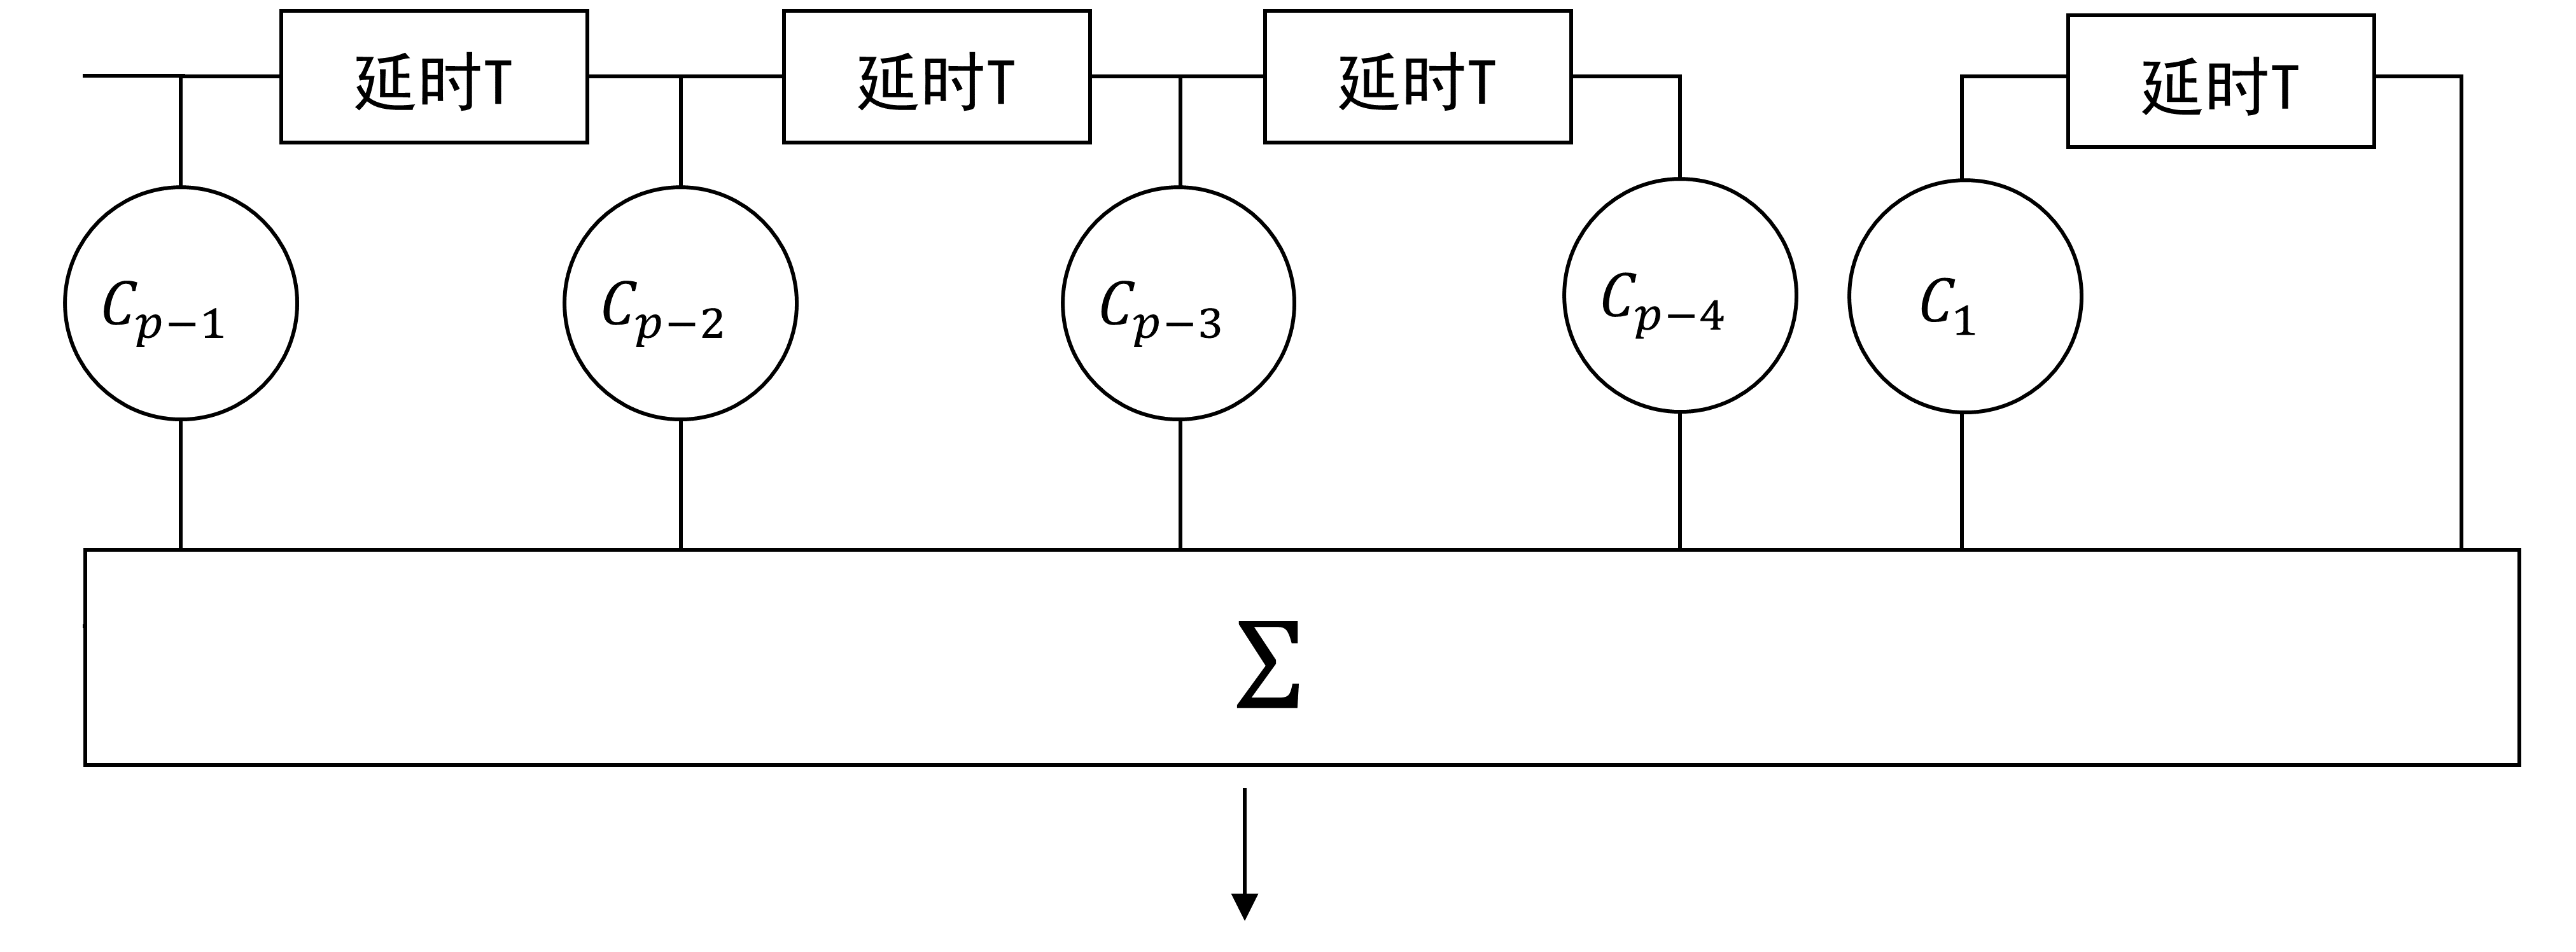
\includegraphics[width=0.8\textwidth]{PPT/5}
  \caption{横向滤波器(即抽头加权延时线求和网络)结构示意图}\label{HXCTJQYSX}
\end{figure}
\subsection{实验步骤}
\begin{enumerate}
  \item 检查实验箱电源以及信号输出的连接方式。
\item 打开实验箱电源以及示波器,调整示波器使观察信号最佳。
\item 按键 K1,数码管显示 P,观察 OUT1 输出的单脉冲信号以及 OUT2输出的匹配滤波信号,记录输出波形。
\item 用示波器测量压缩比、主旁瓣比、码元宽度等参数。
\item 再次按键 K1,改变单脉冲信号码元宽度,LED4 显示带小数点。观察信号 及匹配滤波输出的改变,测量各项参数。
\item 依次按键 K2~K7.选择不同的输入信号,重复步骤 2~4,观察波形,记 录数据。
\item 关闭实验电源,总结实验数据。
\item 记录实验数据数据,进行分析。
\end{enumerate}
\subsection{实验结果}
匹配滤波器测试数据见表\ref{tab:addlabelPPLVQ},对应的波形情况可参加表\ref{tab:PPLVQCSBX2}
。
\begin{table}[htbp]
  \centering
  \caption{匹配滤波器测试数据}
    \begin{tabular}{|c|c|c|c|c|}
    \hline
    序号 & 信号波形 & 码元宽度 & 压缩比 & 主旁瓣比 \\
    \hline
    \multirow{2}[4]{*}{1} & \multirow{2}[4]{*}{单脉冲} & 30us & 1 &   \\
\cline{3-5}      &   & 60us & 1 &  \\
    \hline
    \multirow{2}[4]{*}{2} & \multirow{2}[4]{*}{脉冲串} & 10us & 1 &  \\
\cline{3-5}      &   & 20us & 1 &  \\
    \hline
    \multirow{2}[4]{*}{3} & \multirow{2}[4]{*}{31位M序列} & 1us & 31 &  \\
\cline{3-5}      &   & 2us & 31 &  \\
    \hline
    \multirow{2}[4]{*}{4} & \multirow{2}[4]{*}{31位PN截断码} & 1us & 31 & 16.9dB \\
\cline{3-5}      &   & 2us & 31 & 16.9dB \\
    \hline
    \multirow{2}[4]{*}{5} & \multirow{2}[4]{*}{13位巴克码} & 1us & 13 & 13.98dB \\
\cline{3-5}      &   & 2us & 13 & 13.98dB \\
    \hline
    6 & 4位/7位组合巴克码 & 1us & 28 & 11.6dB \\
    \hline
    \end{tabular}%
  \label{tab:addlabelPPLVQ}%
\end{table}%
\begin{longtable}{|c|c|c|c|}
    \caption{匹配滤波器测试波形}
    \label{tab:PPLVQCSBX2}\\
    \hline
    \multirow{2}[4]{*}{序号}&\multirow{2}[4]{*}{信号}&码元&\multirow{2}[4]{*}{波形}\\
    & &宽度&\\
    \hline
    \endfirsthead

    \hline
    \multirow{2}[4]{*}{序号}&\multirow{2}[4]{*}{信号}&码元&\multirow{2}[4]{*}{波形}\\
    & &宽度&\\
    \hline
    \endhead

    \hline
    \endfoot


    \endlastfoot

   \multirow{2}[4]{*}{1} & \multirow{2}[4]{*}{单脉冲} & 30us &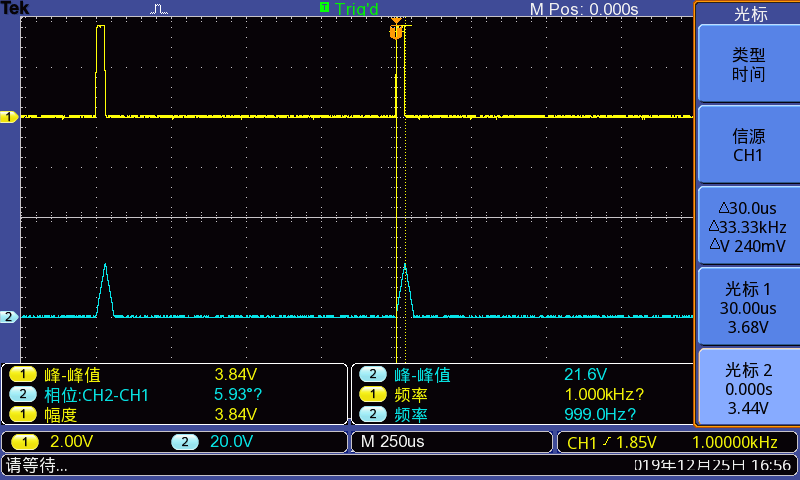
\includegraphics[width=0.45\textwidth]{data/new/F0025TEK}  \\
\cline{3-4}      &   & 60us & 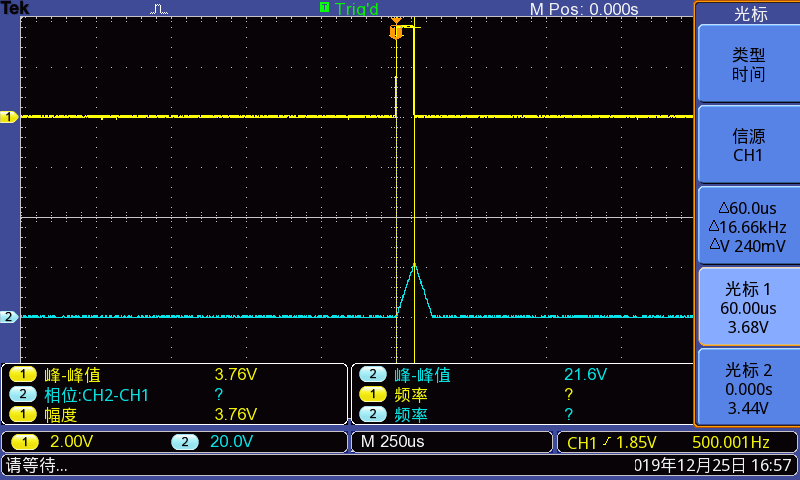
\includegraphics[width=0.45\textwidth]{data/new/F0026TEK}\\
    \hline
   \multirow{2}[4]{*}{2} & \multirow{2}[4]{*}{脉冲串} & 10us & 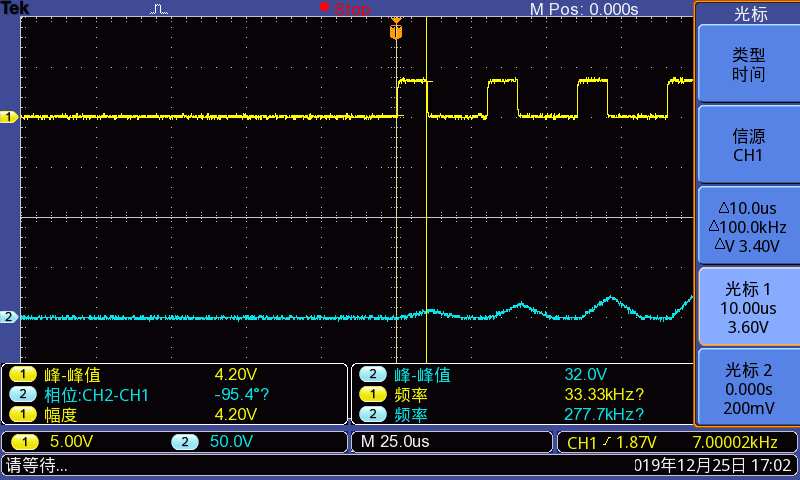
\includegraphics[width=0.45\textwidth]{data/new/F0030TEK}\\
\cline{3-4}      &   & 20us & 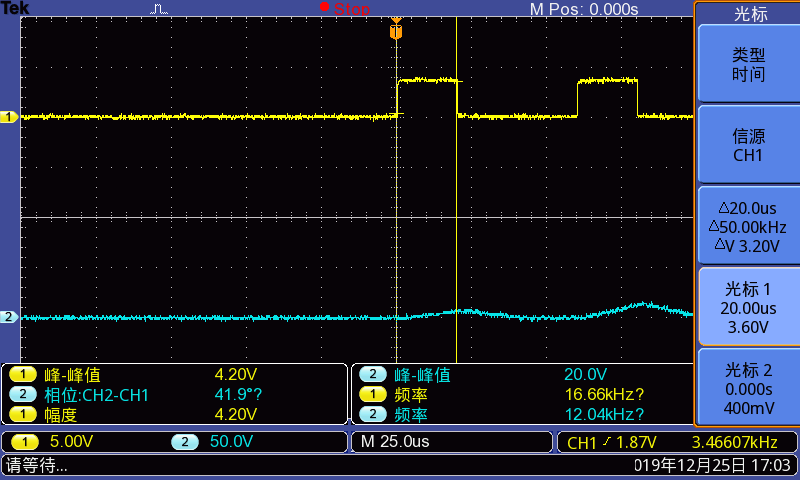
\includegraphics[width=0.45\textwidth]{data/new/F0031TEK} \\
    \hline
3 & 31位M序列 & 1us & 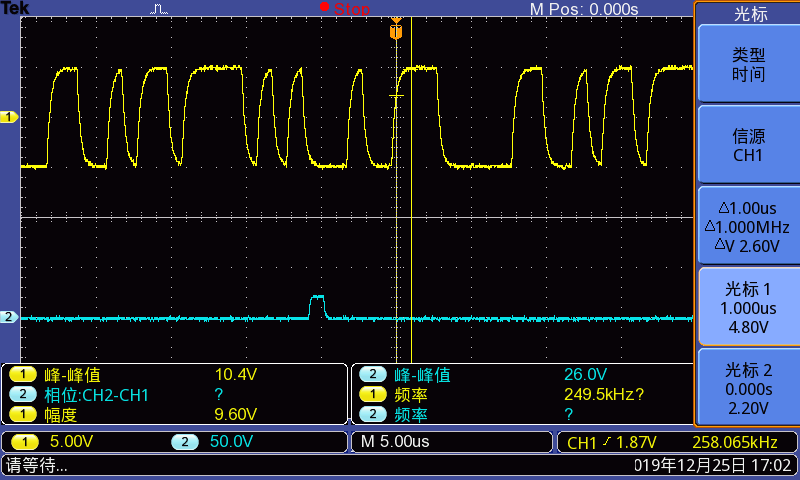
\includegraphics[width=0.45\textwidth]{data/new/F0029TEK}\\
    \hline
    \multirow{2}[4]{*}{4} & \multirow{2}[4]{*}{31位PN截断码} & 1us & 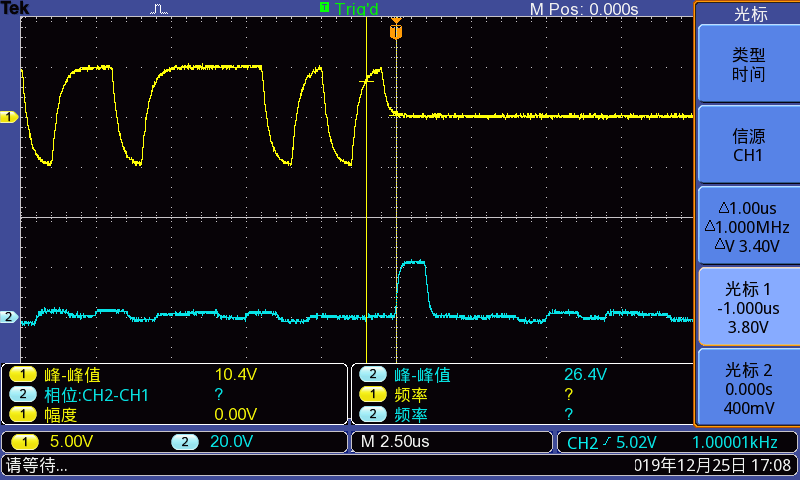
\includegraphics[width=0.45\textwidth]{data/new/F0032TEK} \\
    &&&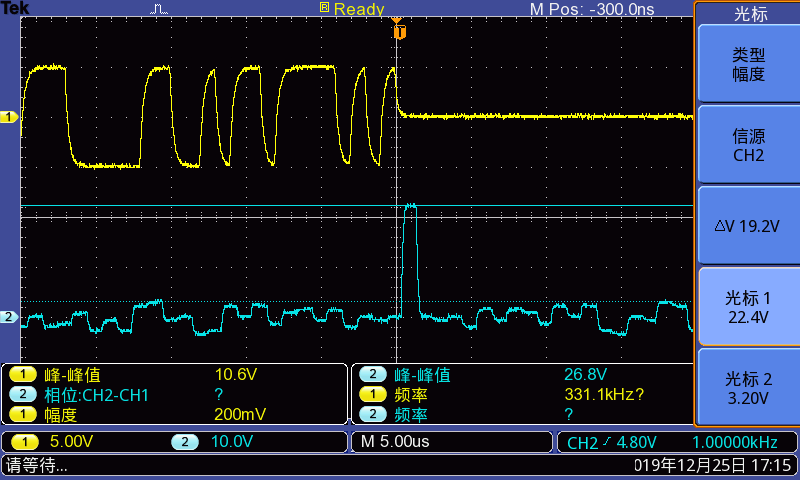
\includegraphics[width=0.45\textwidth]{data/new/F0033TEK}\\
\cline{3-4}      &   & 2us & 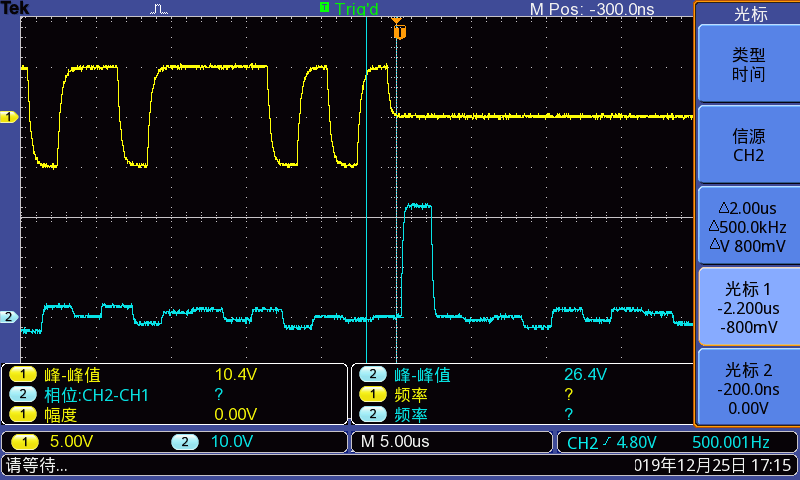
\includegraphics[width=0.45\textwidth]{data/new/F0034TEK} \\
    \hline
5  & 13位巴克码  & 2us & 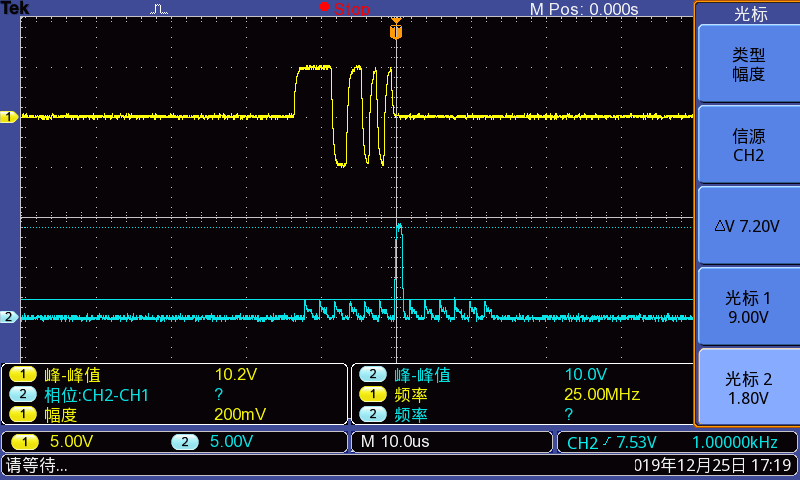
\includegraphics[width=0.45\textwidth]{data/new/F0037TEK}  \\
    \hline
    \multirow{2}[4]{*}{6} & \multirow{2}[4]{*}{4位/7位组合巴克码} & \multirow{2}[4]{*}{1us} &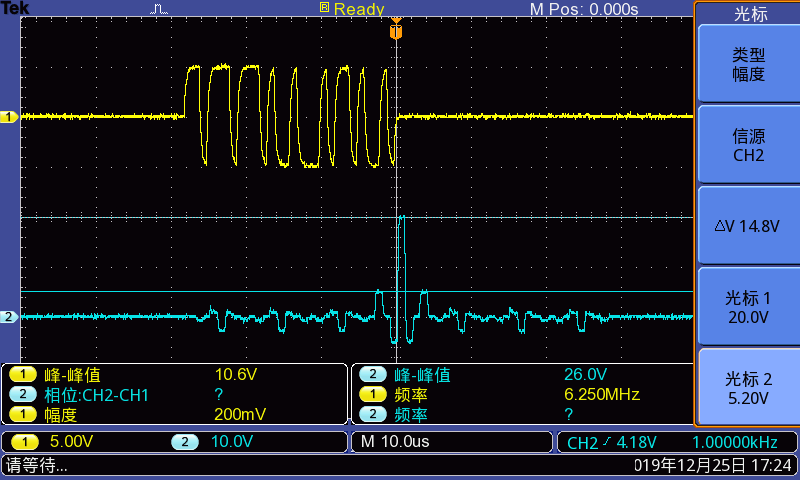
\includegraphics[width=0.45\textwidth]{data/new/F0041TEK}  \\
      &&&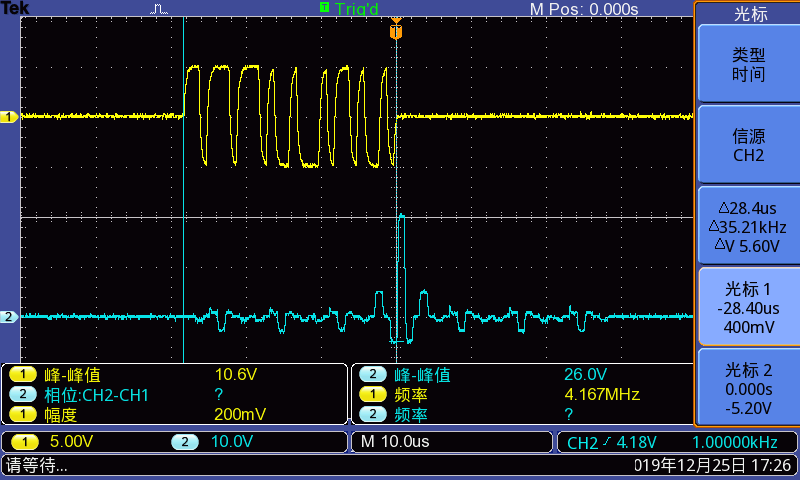
\includegraphics[width=0.45\textwidth]{data/new/F0042TEK}\\
    \hline
\end{longtable}
\subsection{思考题解答}
\begin{enumerate}
  \item \textbf{为什么脉冲压缩输出波形为方波而不是三角波?}\par
因为采用数字信号处理省略了子脉冲匹配滤波器,所以脉压输出的是方波而不是三角波。
\item \textbf{主副瓣比的测量方法有哪些?}\par
方法有:
\begin{enumerate}[(1).]
  \item 通过示波器,测出幅度最大时的电压大小,再测出幅度第二大时的电压大小,两者的比值再换算成分贝,即为主旁瓣比值。
 \item 主旁瓣比=(主瓣-副瓣)$\times$24.2
\end{enumerate}
\item \textbf{31位PN截断码(m序列中截取一个周期)与31位m序列的脉冲压缩输出波形为何不一样?}\par
截断序列是从M序列中截取一个周期所得到的序列,截取后的序列便失去了周期性,而非周期序列的自相关函数没有双电平性,而且截止位置不同的话会得到不同的截断序列码型,所以两者的脉冲压缩输出波形不一样。
\end{enumerate}
\newpage
\section{动目标检测及相参积累}
\setcounter{equation}{0}
\setcounter{table}{0}
\setcounter{figure}{0}
\subsection{实验目的}
\begin{enumerate}
  \item 了解动目标检测(MTD)及相参积累的工作原理。
\item 掌握动目标检测(MTD)及相参积累的性能测试方法。
\end{enumerate}
\subsection{实验仪器}
示波器、万用表。
\subsection{实验原理}
动目标检测(MTD)是利用了动目标雷达回波信号的多普勒频率偏移,采用滤波器组在复杂的雷达回波中检测出运动目标的多普勒频率,并以此来确定动目标的距离、速度和方位。其中,滤波器组具有不同的中心频率,其实质是相当于对不同多普勒通道进行相参积累处理。\par
当杂波功率谱$C(f)$和信号频谱$S(f)$已知时,最佳滤波器的频率响应是:
\begin{equation}
H(f)=\frac{S^*(f)e^{-j2\pi ft_0}}{C(f)}
\end{equation}
这实际上就是基于有色噪声(这里称为杂波)白化处理的匹配滤波器。这一
滤波器可分为两个级联的滤波器和,其传递函数分别为:
\begin{equation}
\begin{array}{c}
  |H_1(f)|^2=\frac{1}{C(f)} \\
  H_2(f)=H_1^*(f)S^*(f)e^{-j2\pi ft_0}\\
\end{array}
\end{equation}
可以粗略的认为,$H_1(f)$用于杂波抑制,而$H_2(f)$用于对雷达回波脉冲串信号匹配。对MTI而言,它要使杂波得到抑制而要让各种速度的运动目标信号通过,所以MTI滤波器即相当于$H_1(f)$;至于和目标信号的匹配,对单个脉冲而言可用中频带通放大器来保证,而对脉冲串则只能采用对消后的非相参积累。所以实际能做到的大多数MTI滤波器,只能使其滤波特性的凹口对准杂波梳状谱的中心,且使二者宽度基本相当。有时也将这称为杂波抑制准最佳滤波。对于相参脉冲串信号$H_2(f)$还可进一步表示成:
\begin{equation}
H_2(f)=H_{21}(f)H_{22}(f)
\end{equation}
即信号匹配滤波器为$H_{21}(f)R$和$H_{22}(f)$两个滤波器级联。式中$H_{21}(f)$为单个脉冲的匹配滤波器,通常由接收机中放实现;$H_{22}(f)$专对相参脉冲串进行匹配滤波,它利用了回波脉冲串的相位特性而进行相参积累;$H_{22}(f)$是梳齿形滤波器,齿的间隔为脉冲重复频率,齿的位置取决于回波信号的多普勒频移,而齿的宽度则应和回波谱线宽度相一致。\par
要对回波相参脉冲串作匹配滤波,必须知道目标的多普勒频移以及天线扫描对脉冲串的调制情况(亦即信号的时宽,对简单信号而言它决定信号的频宽)。实际情况中,多普勒频移不能预知,因此需要采用一组相邻且部分重叠的滤波器组,覆盖整个多普勒频率范围,这就是窄带多普勒滤波器组,如图\ref{DTMBXSHDPLLBQZDTX}
所示。
\begin{figure}[htbp]
  \centering
  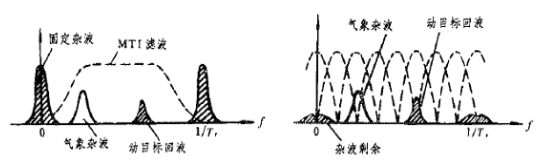
\includegraphics[width=0.8\textwidth]{word/0019}
  \caption{动目标显示和多普勒滤波器组的特性}\label{DTMBXSHDPLLBQZDTX}
\end{figure}\par
从图\ref{DTMBXSHDPLLBQZDTX}
的对比,我们可以看出MTI滤波无法抑制图中具有多普勒频移的气象杂波,气象杂波干扰了动目标信号的检测;但MTD滤波时,气象杂波与动目标回波处于不同的多普勒通道,第5号滤波器通道取出了动目标回波,完全抑制气象杂波对动目标回波的干扰,同时我们也可以初步确定动目标回波的多普勒频移范围。\par
MTD滤波器具有N个输出的横向滤波器,经过各重复周期的不同加权并求和后,即可实现图1所要求的N个相邻的窄带滤波器组,其原理性结构框图如图\ref{MTD}
所示。
\begin{figure}[htbp]
  \centering
  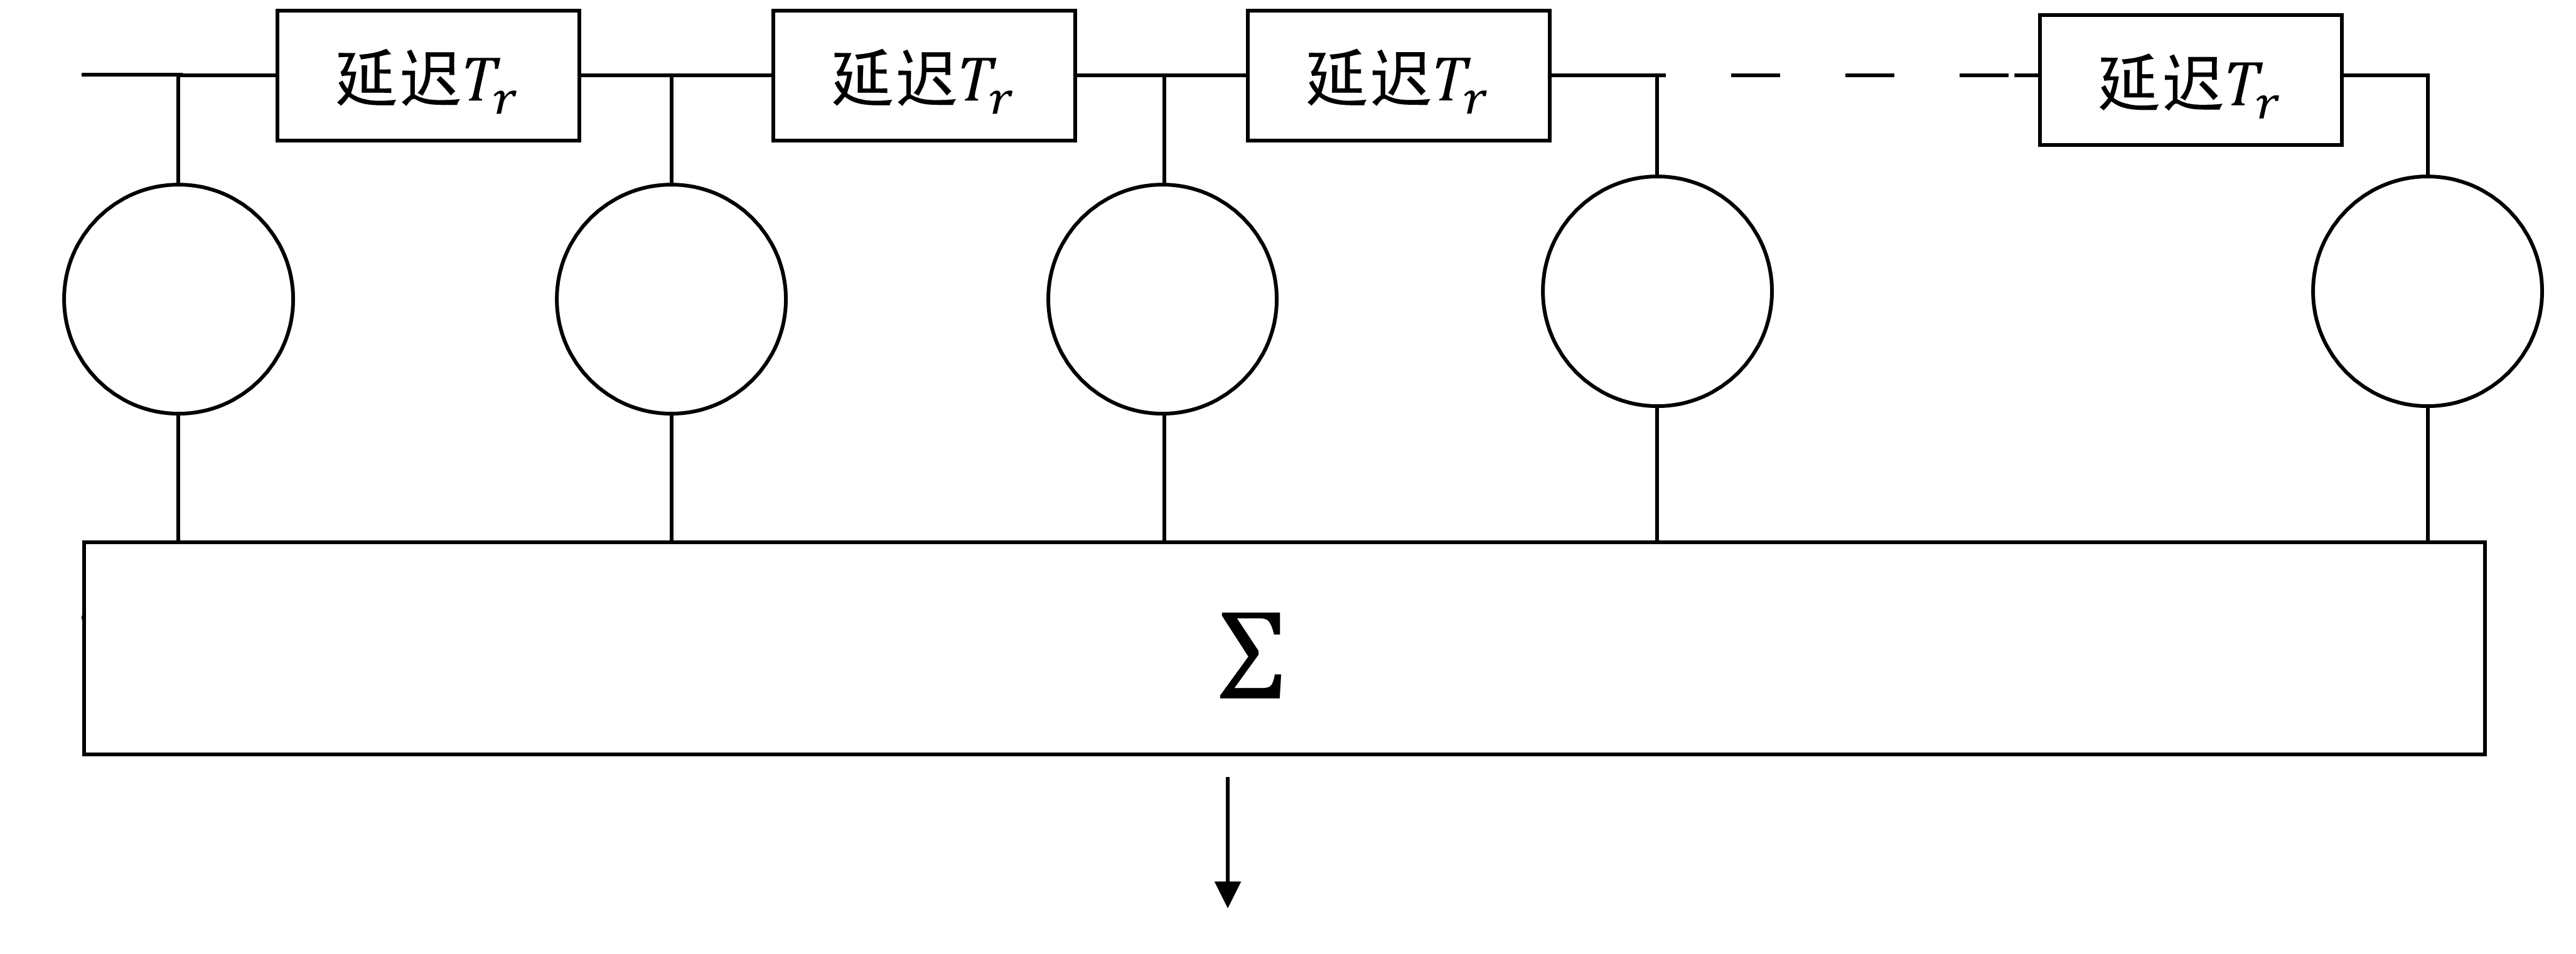
\includegraphics[width=0.8\textwidth]{PPT/6}
  \caption{MTD横向滤波器组结构}\label{MTD}
\end{figure}\par
由于离散傅里叶变换(DFT)是一种特殊的横向滤波器,可以等效成窄带滤波器组,所以若将图2的加权因子按DFT定义选择,并采用DFT的快速算法FFT,就可实现基于FFT的MTD滤波。所以MTD滤波器组既可以在频域利用DFT滤波器组实现也可以在时域采用FIR滤波器两种方法来实现。\par
图\ref{MTDreal}
为实际测量的MTD滤波器特性曲线。图中凹口宽度W1与总底部宽度W2之比定义为凹口相对宽度,它代表了抑制杂波的频谱宽度。越宽则抑制杂波的频谱宽度越宽,杂波抑制性能越好,但盲速越严重,丢失运动目标的可能性越大,信噪比损失越严重;反过来,MTD滤波器凹口相对宽度越窄则抑制杂波的频谱宽度越窄,杂波抑制性能越差,盲速越相对不严重,丢失运动目标的可能性越小,信噪比损失不严重。因此MTD滤波器凹口宽度要折中选择。
\begin{figure}[htbp]
  \centering
  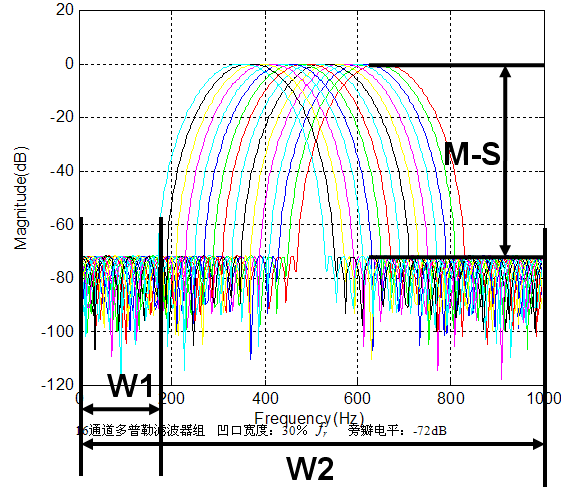
\includegraphics[width=0.5\textwidth]{word/0024}
  \caption{16脉冲MTD实测特性曲线(对数,滤波器组16根曲线叠加在一起)}\label{MTDreal}
\end{figure}
\subsection{实验步骤}
\begin{enumerate}
  \item MTD滤波器副瓣电平测量计算方法\par
  副瓣电平为:$255C\frac{M-S}{F}=96.9\frac{M-S}{F}$\par
  凹口相对宽度为凹口宽度W1与总底部宽度W2之比:$\frac{W1}{W2}$
\item 连接实验装置
\item 测试MTD和FFT特性曲线,并记录数据
\end{enumerate}
\subsection{实验结果}
测试的数据情况见表\ref{tab:addlabelMTD1},对应的波形情况见表\ref{tab:MTDBXT2}
。
\begin{table}[htbp]
  \centering
  \caption{动目标检测及相参积累测试数据}
    \begin{tabular}{|c|c|c|}
    \hline
      & 副瓣电平 & 凹口相对宽度 \\
    \hline
    16点MTD & 73.568 & 0.2 \\
    \hline
    8点MTD & 54.208 & 0.13\\
    \hline
    \end{tabular}%
  \label{tab:addlabelMTD1}%
\end{table}%

\begin{longtable}{|c|c|}
    \caption{动目标检测及相参积累测试波形}
    \label{tab:MTDBXT2}\\
    \hline
    项目&波形\\
    \hline
    \endfirsthead

    \hline
    项目&波形\\
    \hline
    \endhead

    \hline
    \endfoot

\hline
    \endlastfoot

   \multirow{3}[4]{*}{16点MTD} &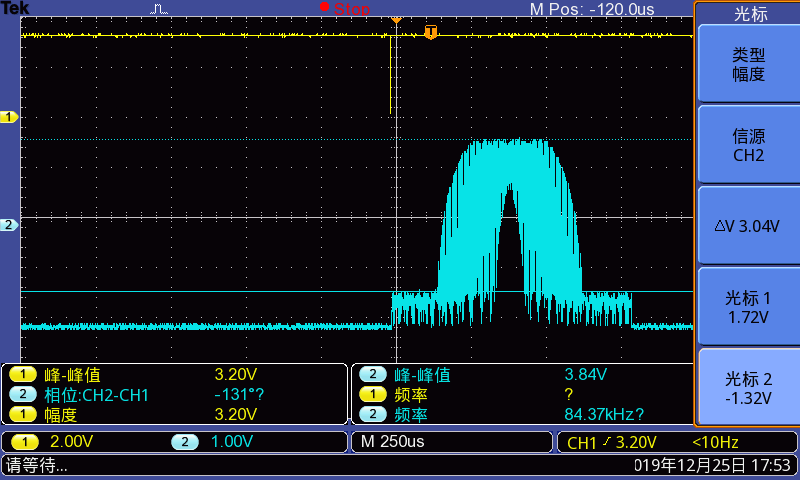
\includegraphics[width=0.45\textwidth]{data/new2/F0010TEK}  \\
   &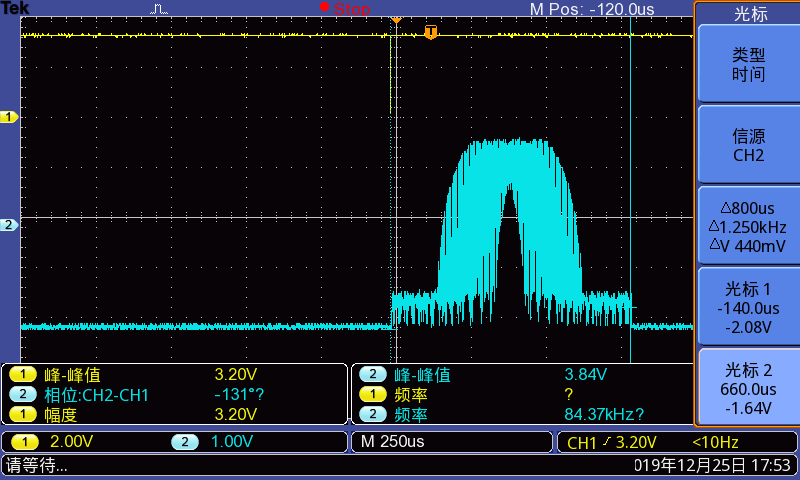
\includegraphics[width=0.45\textwidth]{data/new2/F0011TEK}\\
      &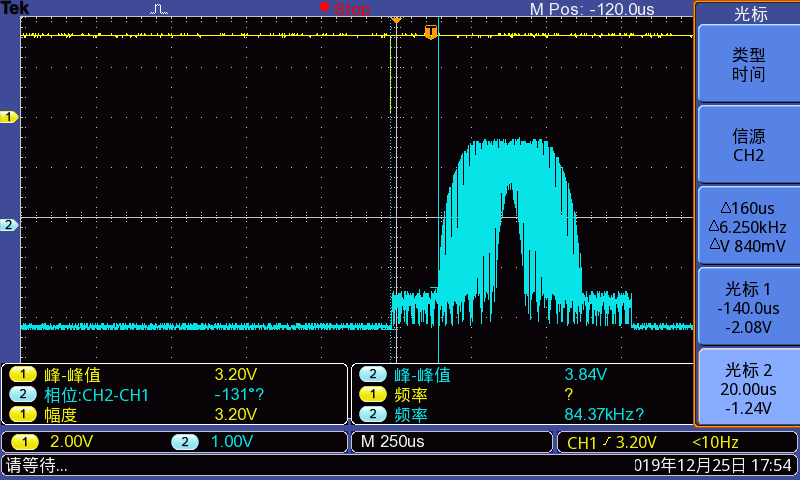
\includegraphics[width=0.45\textwidth]{data/new2/F0012TEK}\\
      \hline
      \multirow{3}[4]{*}{8点MTD} &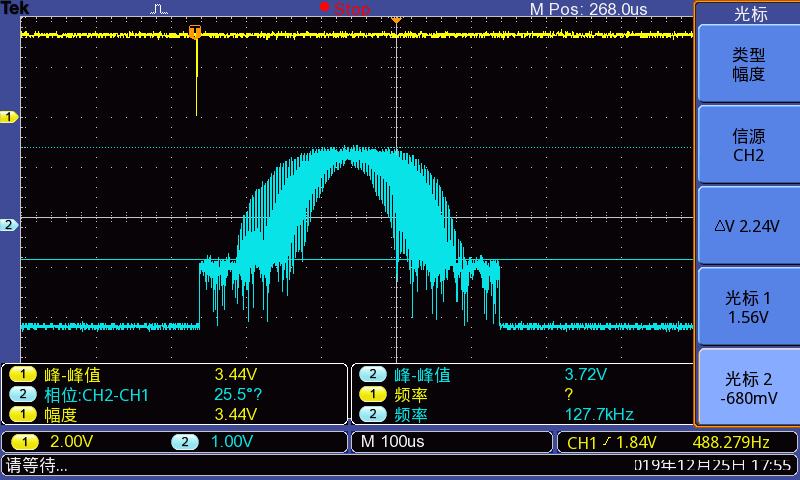
\includegraphics[width=0.45\textwidth]{data/new2/F0013TEK}  \\
      &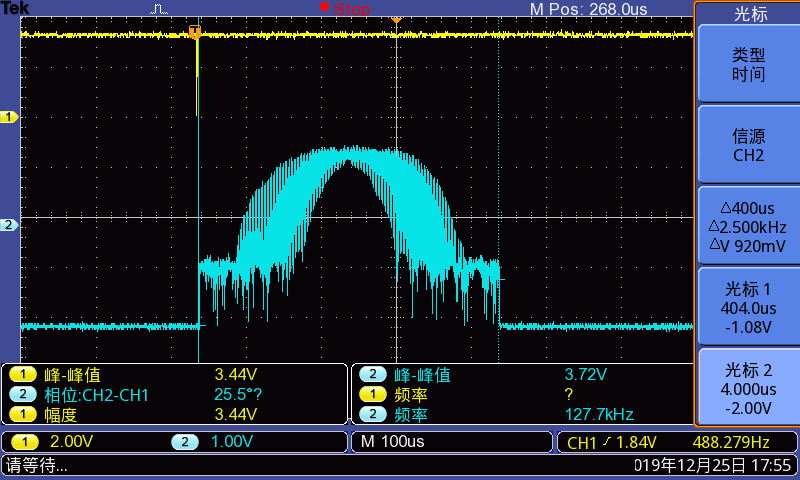
\includegraphics[width=0.45\textwidth]{data/new2/F0014TEK}\\
      &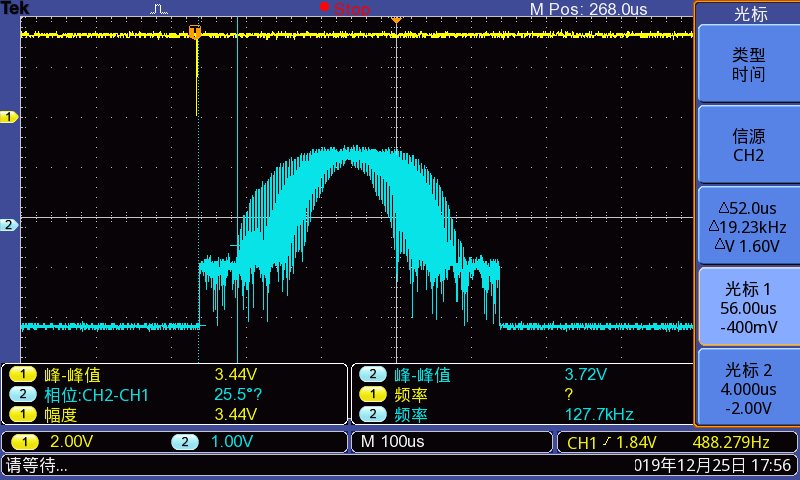
\includegraphics[width=0.45\textwidth]{data/new2/F0015TEK}\\
      \hline
\end{longtable}
\subsection{思考题解答}
\begin{enumerate}
  \item \textbf{为什么FFT等效于脉冲相参积累?}\par
  FFT的信号处理是在频率里对信号处理的。具有N个输出的横向滤波器经过各重复周期的不同加权并求和后,实现N个相邻的窄带滤波器组。全部滤波器响应覆盖了从0到$f_r$的频率范围,输入信号经延迟排列等待:当信号全部输入完毕才同时输出,这样相参的信号幅度叠加输出为最大值、不相差信号则幅度相近,经过该滤波器后,它将N个相参信号积累,使信噪比提高N倍。因此,FFT等效于脉冲相参积累。
  \item \textbf{为什么要加权,如何选择窗函数?}\par
  加权是为了抑制旁瓣及把旁瓣电平降低,使得弱目标回波能够检测出来。FFT滤波器组各个滤波器的旁瓣较高,阻带衰减小,对数据进行加窗处理,降低旁瓣电平,但压低副瓣的同时加宽了主瓣并引起了失配损失。\par 目前常用的窗含数主要有汉宁窗,海明窗,布莱克曼窗,泰勒窗,切比雪夫窗等。\par 要求窄的主瓣和低的副瓣是矛盾的,折中考虑,海明窗的综合性能最佳。但具体使用哪个窗函数则要视具体情况而定。
  \item \textbf{FFT+MTI方法实现MTD与FIR滤波器组实现MTD有何区别?}\par
  FFT滤波器组在零频附近没有足够的凹陷,无法很好的抑制地物杂波,在FF滤波器组之前加上MTI处理,先抑制地物杂波,来改善检测性能。这种方法运算量少速度快。\par
  FIR横向滤波器形式可以灵活设计每个滤波器的权系数,使其幅度频率响应都在零频附近有较深的凹陷,用于抑制地杂波。具有灵活性高、运算控制简单,可根据杂波设计自适应和杂波抑制能力强等优点。\par
  FFT是在频率对信号进行处理,输出为延迟波形;而FIR是在时域对信号处理,输出是实时波形。
\end{enumerate}
\appendix
\section{利用MATLAB复现数据波形}
\setcounter{section}{4}
\setcounter{equation}{0}
\setcounter{table}{0}
\setcounter{figure}{0}
\subsection{复现原理}
示波器将波形以图片形式保存在U盘的同时,也将波形数据信息保存在了一起。调用数据信息借助MATLAB的绘图工具绘图即可。
\subsection{MATLAB代码}
\begin{lstlisting}
clc;close all;clear all;
M=42 %第M个保存的数据
A = xlsread(['E:\baogao\data\ALL00',num2str(M),'\F00',num2str(M),'CH1.csv']);%数据存储位置
B = xlsread(['E:\baogao\data\ALL00',num2str(M),'\F00',num2str(M),'CH2.csv']);
x1=A(:,3);
y1=A(:,4);
x2=B(:,3);
y2=B(:,4);
figure(1)
subplot(2,1,1)
plot(x1,y1,'r');
axis tight;
figure(1)
subplot(2,1,2)
plot(x2,y2,'b');
axis tight;
\end{lstlisting}
\subsection{部分复现数据与示波器图片对比}
部分复现的数据与示波器图片对比见表\ref{FXSJDB}
\begin{longtable}{|c|c|}
    \caption{部分复现数据与示波器图片对比}
    \label{FXSJDB}\\
    \hline
   复现数据&示波器波形\\
    \hline
    \endfirsthead

    \hline
    复现数据&示波器波形\\
    \hline
    \endhead

    \hline
    \endfoot

\hline
    \endlastfoot

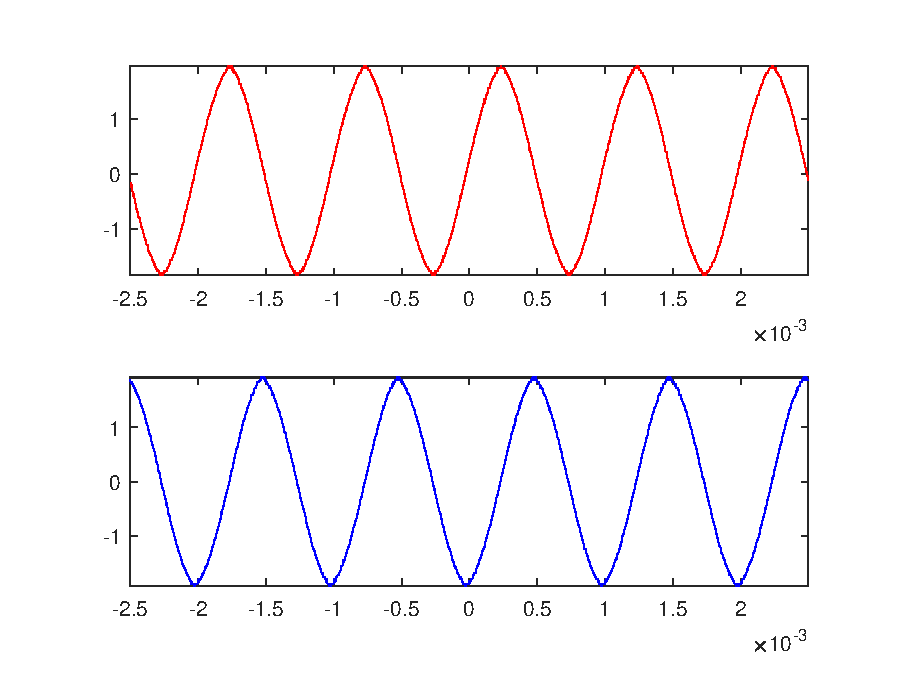
\includegraphics[width=0.45\textwidth]{rebuild/001}&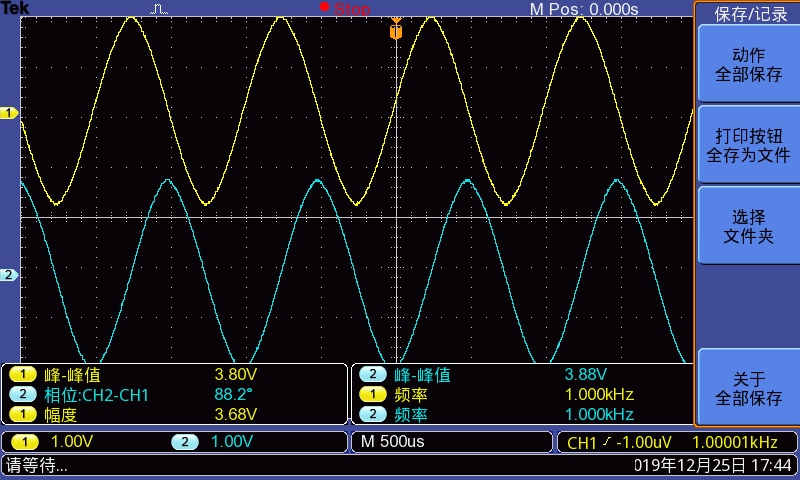
\includegraphics[width=0.45\textwidth]{data3/new/F0007TEK}\\ \hline
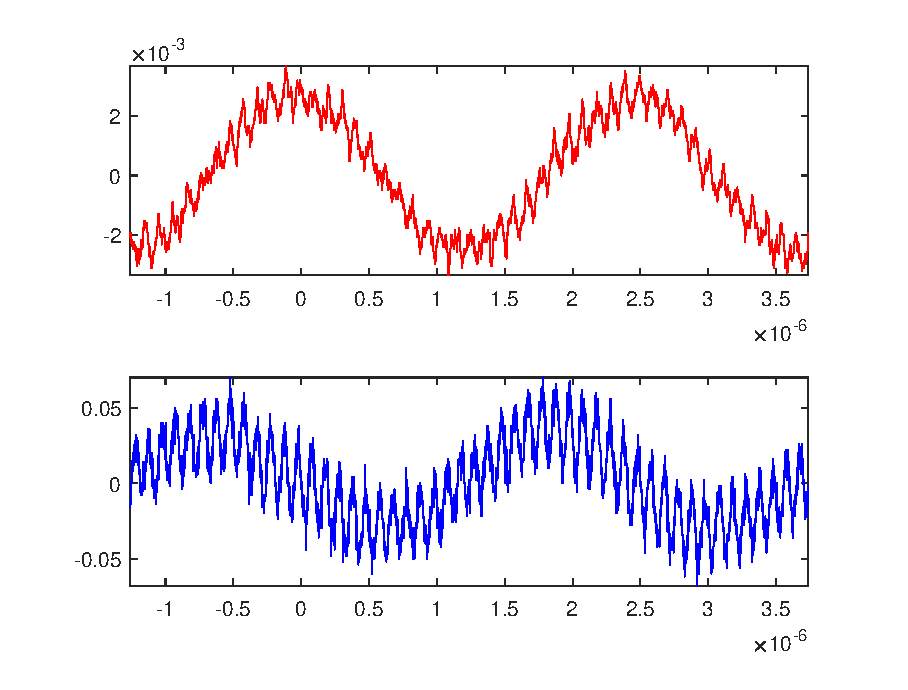
\includegraphics[width=0.45\textwidth]{rebuild/002}&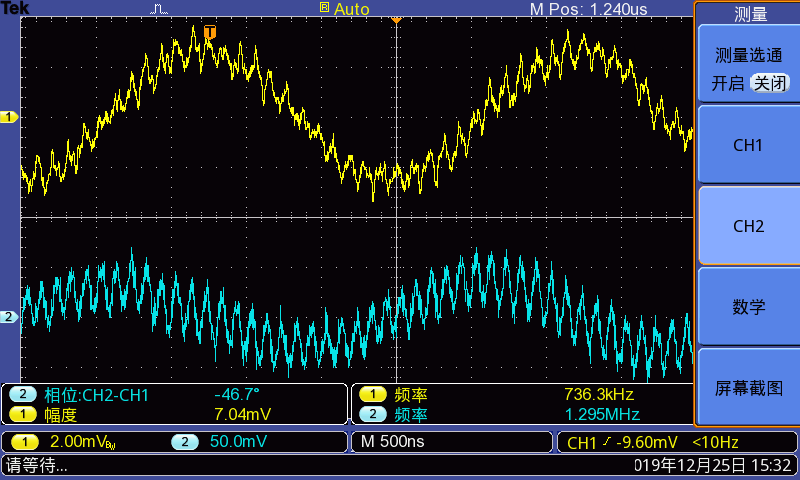
\includegraphics[width=0.45\textwidth]{data3/new2/F0011TEK}\\ \hline
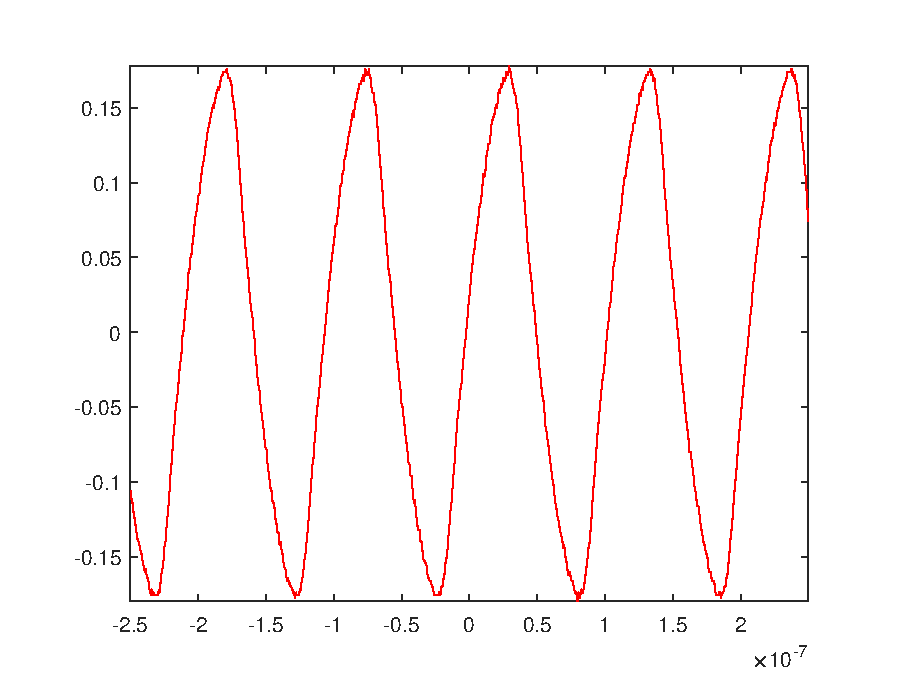
\includegraphics[width=0.45\textwidth]{rebuild/003}&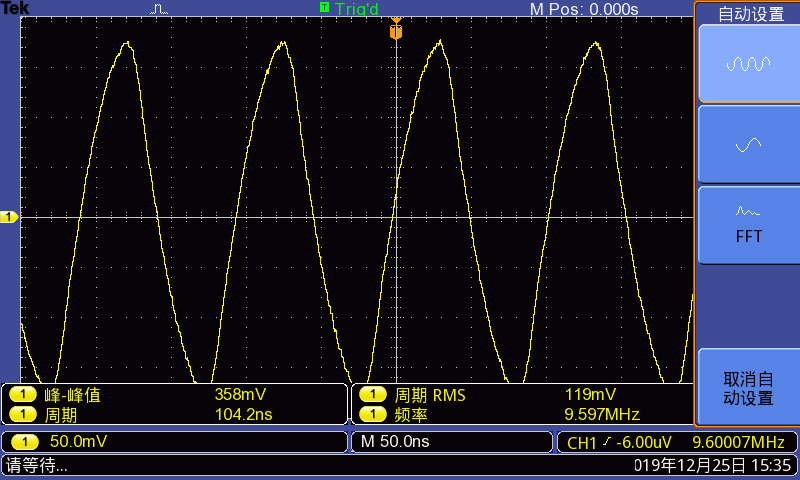
\includegraphics[width=0.45\textwidth]{data3/new2/F0013TEK}\\ \hline
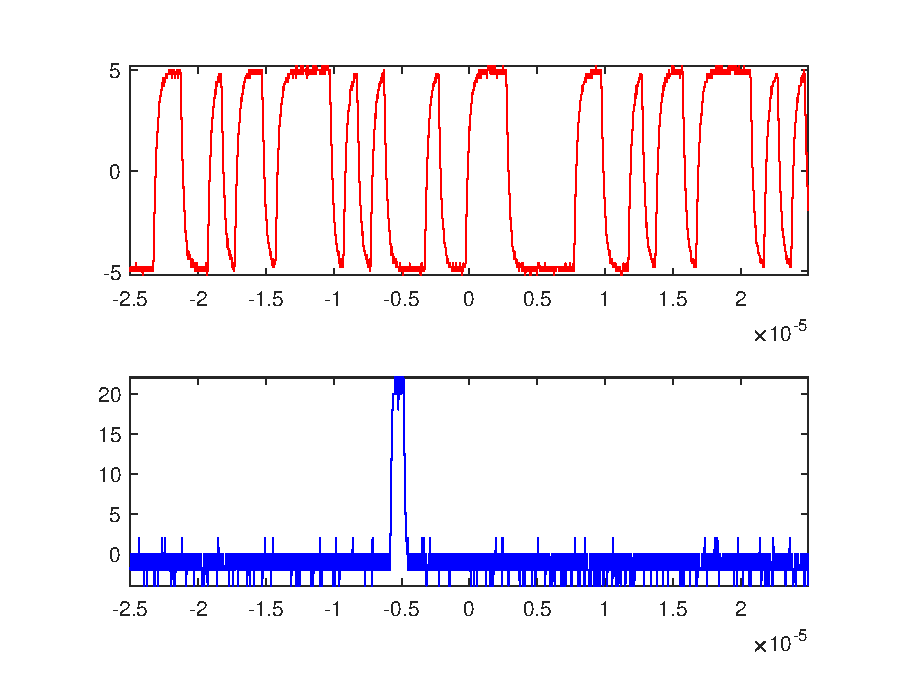
\includegraphics[width=0.45\textwidth]{rebuild/004}&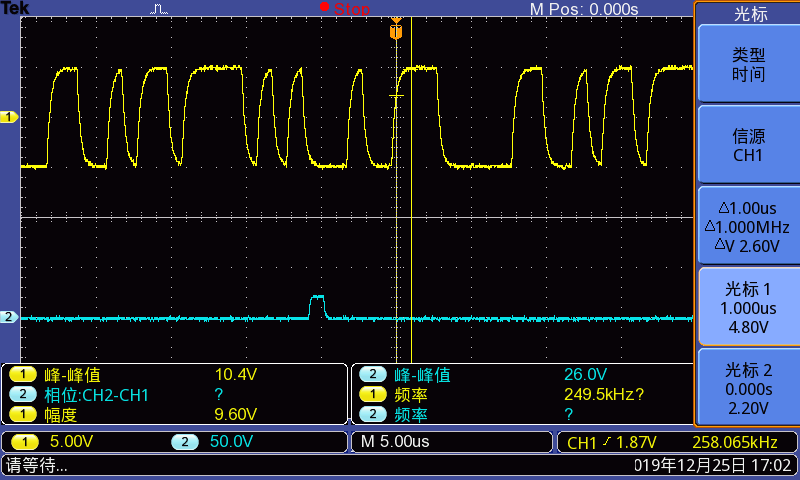
\includegraphics[width=0.45\textwidth]{data/new/F0029TEK}\\ \hline
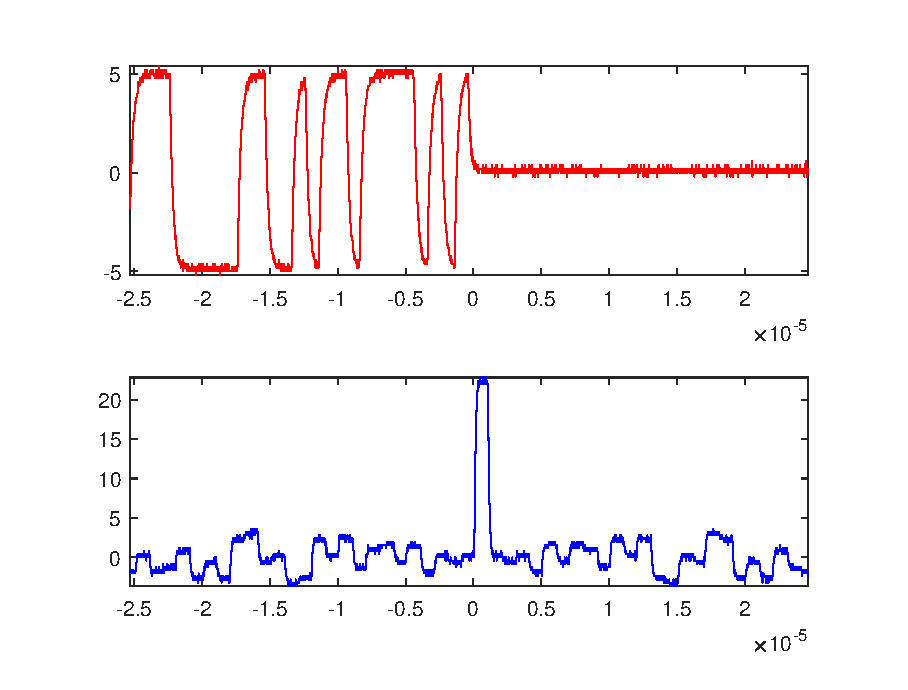
\includegraphics[width=0.45\textwidth]{rebuild/005}&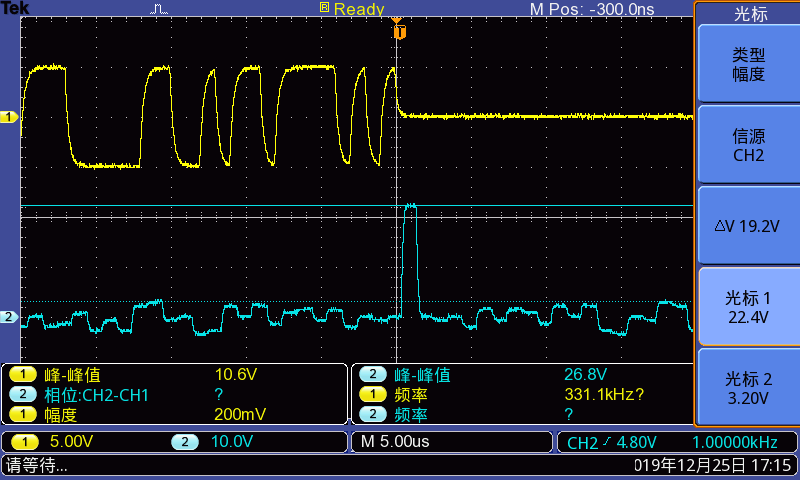
\includegraphics[width=0.45\textwidth]{data/new/F0033TEK}\\ \hline
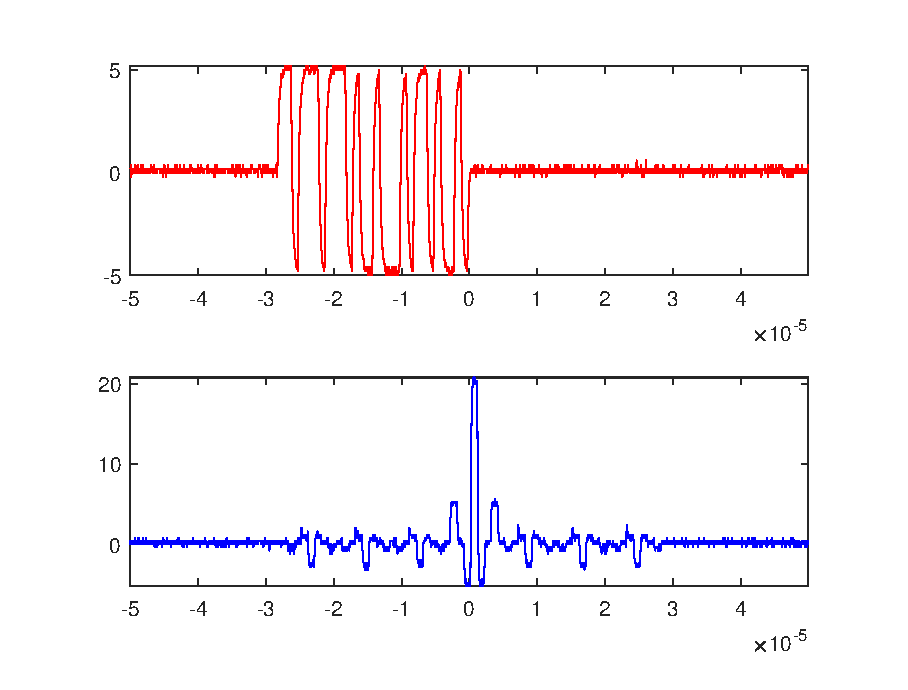
\includegraphics[width=0.45\textwidth]{rebuild/006}&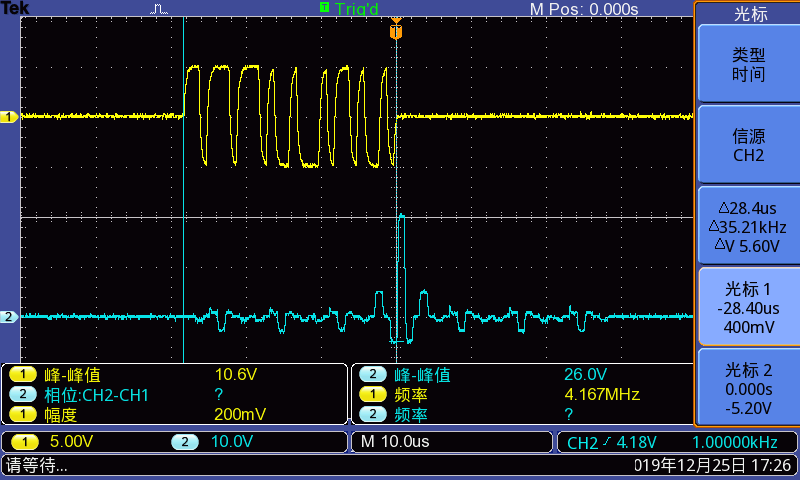
\includegraphics[width=0.45\textwidth]{data/new/F0042TEK}\\ \hline
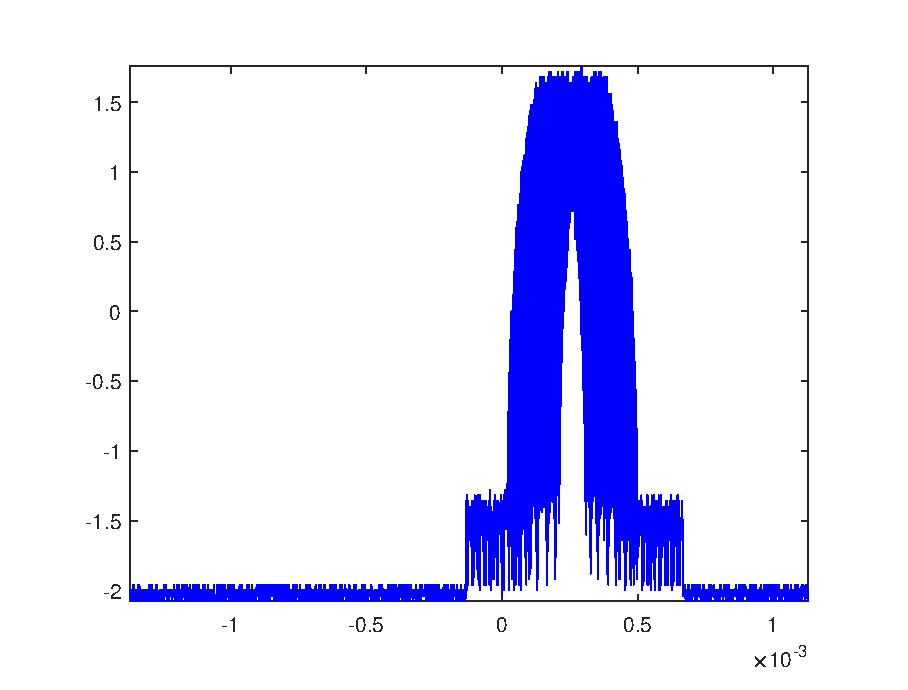
\includegraphics[width=0.45\textwidth]{rebuild/007}&\includegraphics[width=0.45\textwidth]{data/new2/F0010TEK}\\ \hline
\includegraphics[width=0.45\textwidth]{rebuild/008}&\includegraphics[width=0.45\textwidth]{data/new2/F0013TEK}\\ \hline
\end{longtable}
\end{document}
